\documentclass[12pt]{report}
\usepackage[francais]{babel}
\usepackage[utf8]{inputenc}
\usepackage{graphicx}
\usepackage{caption}
\usepackage{amsmath}
\usepackage{hyperref}
\usepackage[section]{placeins}
\addtolength{\hoffset}{-1cm}
\addtolength{\textwidth}{2cm} 
\addtolength{\voffset}{-1cm}
\addtolength{\textheight}{2cm} 


\begin{document}

\begin{titlepage}
\begin{center}

\hfill

\bigskip
\huge{Mémoire  : Projet de Programmation} 
\vfill
\bigskip 
\Huge 
\bigskip Génération automatique de texte \par 
\vfill
\Large Benoît Barthés \par 
		Alexis Boumera \par 
		Baptiste Guiomar \par 
		Claire Pennarun \par 
		Adrien Wintringer
\vfill
\Large Bordeaux 1 \par \Large Projet de Programmation		
		\bigskip 
\bigskip

\Large
\today
\end{center}
\end{titlepage}

\tableofcontents
\newpage

\chapter{Présentation du sujet}

\section{Présentation du domaine}

	Depuis l'apparition des ordinateurs dans les années 50, la question de la reproduction du langage naturel a toujours été une des plus épineuses. \par 
	En effet, le langage humain comprend une multitude de paramètres qui ne sont pas évidents à mettre en oeuvre en termes de programmation : syntaxe, grammaire, intonation, structuration de la pensée... Mais à quoi pourrait bien servir un ordinateur possédant le langage, puisqu'il ne possède pas la pensée, l'intention ; à quoi sert-il de savoir \emph{parler} si l'on ne sait rien \emph{dire} ?

	La question est donc de savoir quoi faire dire à un logiciel, quel texte lui faire générer, et de quelle manière.
	\bigskip 
	
	La génération automatique de texte est surtout un domaine où la machine doit savoir faire beaucoup de choix : choix du sujet à traiter, choix du vocabulaire à employer, choix de l'articulation des phrases... Tous ces choix doivent donc être guidés par le linguiste ou l'informaticien responsable du projet.
	
	\bigskip 
	Les données analysées par le logiciel peuvent être de plusieurs types : tableaux de données financières (comme dans le système EasyText \cite{Dan11}), données statistiques ou météorologiques... Le traitement et l'analyse de données contenues dans une base de données est, par contre, un sujet qui a été très peu, voire pas traité dans le domaine de la génération de texte, sûrement en raison de la difficulté qu'il y a à extirper le sens de telles données.
	
	Quant à la manière utilisée dans la génération de texte elle-même, elle peut également fortement varier : elle peut faire intervenir (ou non) un utilisateur externe, notamment pour l'étape de sélection du contenu pertinent dans les données initiales.


\section{Présentation du projet}

Le but du projet est de réaliser un logiciel permettant de générer du texte de manière automatique à partir de données brutes sélectionnées dans une base de données. 

Pour se faire, nous utilisons le logiciel Syntox, qui est un logiciel développé par M. Lionel Clément, et qui génère du texte grammaticalement et syntaxiquement correct à partir d'une entrée d'une forme spécifique (dite \emph{entrée Syntox} dans notre rapport).
Syntox contient à l'avance une grammaire et un lexique qui correspondent au thème traité, ces deux composants étant fournis par M.Clément.

Le but de notre logiciel est donc de fournir à Syntox une entrée qui est ensuite transformée en texte.

\bigskip

Ce logiciel peut servir par exemple à analyser automatiquement des données contenues dans une base de données, ou à utiliser ces données intelligemment pour effectuer des tâches répétitives, notamment l'écriture de textes demandant une grande adaptation des termes suivant les situations (on peut penser au mailing automatique pour des commerciaux ou pour une administration, qui doivent adapter leur message à tous les types de destinataires).

La base de données considérée dans ce projet est une base de données relationnelle, contenant des informations intéressantes pour l'utilisateur, mais non exploitables directement ; il s'agit de données chiffrées, de fonctions, de relations, qui doivent être étudiées avant d'être interprétées.

\bigskip

La génération du texte se fait à partir de \emph{scénarios utilisateur} : chaque scénario correspond à un but rhétorique visé par l'utilisateur.

Notre logiciel fait donc intervenir un utilisateur, qui peut construire le scénario voulu à partir de \emph{concepts} : ceux-ci peuvent être une action, un événement, une succession, un objet, une personne... Le concept est complètement indépendant de la manière de le représenter (notamment indépendant du lexique utilisé, et même de la langue).

Les concepts dits "simples" ou atomiques, sont en général les personnes, ou les objets (ce qui correspond souvent aux noms propres ou aux noms communs). Dans l'exemple ci-dessous, les concepts "match" et "équipe" sont des concepts simples.

Par exemple, le concept "Gagner\_Match" peut être représenté ainsi :
$$\begin{bmatrix}
\text{Gagner\_match} \\ \text{arg1 = équipe} \\ \text{arg2 = match}
\end{bmatrix}
$$
Les arguments d'un concept peuvent être eux-mêmes des concepts : cela permet de fabriquer des concepts plus complexes.
Par exemple, le concept de causalité prend en argument deux concepts, qui sont complexes :

$$\begin{bmatrix}
\text{cause} \\ \text{arg1 = antécédent} \\ \text{arg2 = conséquence}
\end{bmatrix}
$$

Dans notre projet, le logiciel propose à l'utilisateur de choisir entre la création d'un nouveau scénario (et l'utilisateur devra alors choisir les concepts qu'il veut exprimer, ainsi que leurs arguments) et la réutilisation d'un scénario déjà établi et sauvegardé.

\bigskip


Le scénario (c'est-à-dire l'ensemble de concepts plus ou moins complexes que l'utilisateur veut exprimer) est ensuite traité en plusieurs étapes par le logiciel pour générer l'entrée Syntox souhaitée.

Premièrement, le scénario est transformé en un \emph{graphe conceptuel}, c'est-à-dire un graphe acyclique orienté dont les sommets sont des concepts et les arêtes orientées correspondent aux liens entre ces concepts.

Exemple de graphe conceptuel :
\begin{figure}[!h]
\begin{center}
	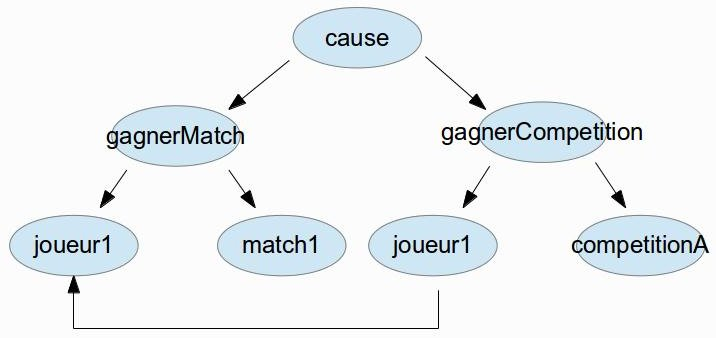
\includegraphics[scale=0.5]{graphe_cause.png}
	\caption{La victoire du joueur1 dans le match1 entraîne sa victoire de la compétition A.}
\end{center}
\end{figure}

Ce graphe est ensuite parcouru pour le retranscrire en entrée Syntox.

Par exemple, le graphe ci-dessus provoque la génération de l'entrée suivante :
\begin{verbatim}
   S Axiom[PRED=cause,
      arg1=[PRED=gagnerMatch, 
           tense=present, 
           subj=[PRED=joueur1, number=sg, def=+],
           obj=[PRED=match1, number=sg, def=+]],
      arg2 =[PRED=remporterCompetition,
           tense=present,
           subj=[PRED=joueur1, number=sg, def=+],
           obj=[PRED=competition, number = sg, def=+]]
\end{verbatim}

Chaque entrée permet à Syntox de générer toutes les phrases correspondant aux contraintes qui y sont spécifiées.

Dans notre exemple, Syntox génère alors les phrases :

\begin{enumerate}
    \item le joueur1 gagne le match1 , par conséquent le joueur1
remporte la compétition .
	\item le joueur1 gagne le match1 . le joueur1 remporte la
compétition .
	\item le joueur1 gagne le match1 , donc le joueur1 remporte
la compétition .

\end{enumerate}

On récupère ces phrases, qui correspondent au texte voulu par l'utilisateur. 
Celui-ci peut ensuite enregistrer le résultat dans un fichier.

\bigskip

Notre logiciel comporte deux types d'utilisateurs : l'utilisateur dit "classique", qui ne se préoccupe pas de la manière dont le texte est généré, et l'utilisateur administrateur, qui peut configurer le système.

Ainsi, l'administrateur peut configurer le système (créer les concepts requis et donner les informations de connexion à la base de données), puis l'utilisateur classique n'a plus qu'à utiliser le logiciel, sans avoir besoin de connaître la base de données utilisée ou les détails des concepts qu'il manipule.


\chapter{Etude de l'existant et bibliographie}

\section{Eléments bibliographiques}

L'état de l'art \cite{Bat93} présenté par John Bateman en 1993 (et mis à jour régulièrement depuis) concernant la génération automatique de texte est une base de connaissances très importante pour nous. En effet, l'auteur reprend les avancées des travaux les plus importants dans ce domaine, enrichi d'une grande bibliographie. Il donne également des méthodologies précises pour traiter des problèmes de la génération automatique de texte.
Cet état de l'art, assez conséquent, nous permettra de trouver des références rapidement, même si le sujet que nous traitons n'a pas encore fait l'objet d'une étude poussée.


La synthèse du domaine faite par Laurence Danlos (\cite{Dan00}) est d'un grand intêret pour notre projet. En effet il nous présente de façon très concise ce qu'est la génération automatique de texte. Le premier point intéressant concerne les questions qui se posent généralement dans les applications mettant en oeuvre de la génération de texte, "Quoi dire ?" et "Comment le dire ?". Ce seront probablement des questions que nous aurons à nous poser par la suite. Le document met aussi en avant les différents problèmes et difficultés rencontrés par les sytèmes existants et auxquels nous pourrions avoir à faire face, mais aussi les avantages de tels systèmes. Il est par exemple question de leur "spécialisation" à certains domaines (comme la météo, les finances etc) qui leur permet de ne couvrir qu'une partie de la grammaire et du lexique et d'être ainsi relativement performants. Nous sont aussi présentés dans ce document les différents types d'applications déjà existantes, comme TA(O) (première application développée) ou encore PostGraphe (utilisé dans le domaine statistique). Plus intéressant encore, ce document nous décrit ce que peuvent ou pouraient apporter ces systèmes, comme par exemple une sortie orale (si nous couplions un générateur à une synthétiseur vocal). Une présentation précise des mécanismes et tâches mis en oeuvre dans la génération automatique nous est aussi offerte, avec pour chaque étape une présentation des entrées/sorties. Le document nous présente enfin le problème de l'évaluation de tels systèmes, qui s'avère difficile à résoudre de par leur complexité.

\subsection{EasyText}
Le système de génération de textes EasyText \cite{Dan11} a été développé par Frédéric Meunier, Laurance Danlos, et Vanessa Combet dans le cadre d'une collaboration avec la filliale française Kantar Media de TNS-Sofres. Ce logiciel permet de créer un commentaire à partir d'un tableau de chiffres. 

Contrairement à d'autres procédés de génération de textes tel que les textes à trous ou le publipostage, EasyText utilise un formalisme G-TAG. Ce dernier permet "de transformer une représentation conceptuelle d'un ensemble d'informations en un texte" (d'après Laurence Danlos, \cite {Dan10}). 

\bigskip

Plusieurs étapes ont lieu afin de réaliser le commentaire. Elles se schématisent par deux questions principales: "Quoi dire ?" et "Comment le dire ?" . Dans une première étape il faut sélectionner les informations que l'on peut dire : ce choix se fait en fonction des éléments intéressants présents dans le tableau. On obtient alors une conjonction de formules logiques, qui est ensuite transformée en un texte, en deux temps.

On cherche en premier lieu à transformer la conjonction en phrases (macro-planifi-cation).  On s'appuie alors sur des connaissances rhétoriques et linguistiques de la langue pour structurer l'ordre du texte et déterminer ainsi le "schéma" de la phrase. Enfin, on complète la phrase pour la former selon les conventions de la langue (micro-planification). Pour cela, en fonction du "schéma" auquel elle se rapporte, on ajoute des déterminants, des compléments, etc en prêtant attention à la position à laquelle ils se situent. On s'appuie ici sur des connaissances sémantiques et syntaxiques.  À la suite de toutes ses étapes on obtient un texte formé selon les critères de la langue qui a pour objet les éléments du tableau. 


\section{Etude de l'existant}

\subsection{Projet GAT-2}

Le logiciel GAT-2 (Génération Automatique de Texte 2) \cite{GAT2} est le prédécesseur de notre objectif de travail actuel. Développé l'année dernière par 5 étudiants de master 1 Informatique, il repose principalement sur GAT-1 (développé lui aussi par des étudiants de master 1 Informatique) et sa version améliorée Syntox développée par Lionel Clément: ces deux outils ne se chargent pas du "quoi dire" mais du "comment le dire", prenant en entrée des règles de grammaires énoncées de manière précise et générant un texte fini et syntaxiquement correct.

GAT-2, dans sa version finale, traite simplement une requête SQL énoncée par l'utilisateur (ou plutôt choisie dans une liste prédéfinie par les concepteurs), et y répond via une phrase rédigée en français. Pour ce faire, il se connecte à la base de données, et traite via des opérations logiques simples la requête afin d'en extraire et d'en déduire plusieurs résultats, qui sont formatés de façon à pouvoir être interprétés par GAT-1 qui se charge d'écrire les données répondant à la requête initiale de l'utilisateur en plein texte.
Cependant, il n'arrive pas pleinement à extraire le "sens" (au sens le plus strict du terme) de la base de données, se limitant à la réponse d'une seule question à la fois de manière assez redondante.

\subsection{Syntox}

% A remanier

Syntox \cite{Clem12} est un logiciel développé par Lionel Clément, chercheur au LaBRI dans l'équipe Méthodes Formelles.

Il est défini par son auteur comme un synthétiseur de texte. C'est un type de programme plutôt récent, il en existe donc peu et sont pour la plupart le fait d'universitaires.

Syntox permet de générer du texte à partir de concepts. En d'autres termes il ne vérifie pas qu'une phrase est correcte dans un langage donné, mais il crée une phrase correcte dans une grammaire et un lexique défini à partir d'idées.

Syntox ne se limite donc pas à la génération d'une unique phrase, et peut générer des paragraphes entiers. Sa limite principale se trouve dans les reprises sémantiques comme les anaphores, ou les ellipses.
A l'heure actuelle, le projet représente deux ans de travail.

Son interface utilisateur est accessible via un navigateur web pour permettre de porter les efforts sur le programme en lui même et de ne pas perdre du temps à créer des exécutables pour différentes plateformes. 


\chapter{Cahier des charges}


\section{Scénarios d'utilisation}

\subsection{Scénarios utilisateur}

\subsubsection{Scénario 1}
	\begin{enumerate}
	\item L'utilisateur se connecte en choisissant le mode "Utilisateur" ne requérant pas de mot de passe.
			\item Il sélectionne le projet sur lequel il souhaite travailler, et entre le mot de passe de la base de données correspondante (si il y en a un).
            \item Il choisit "Scénario existant" et dans la liste déroulante il choisit celui qui lui convient en fonction de la base de données active.
            \item Il clique sur le bouton "Valider" pour lancer l'exécution du logiciel.
            \item L'utilisateur peut alors voir le résultat généré par le logiciel.
            \item L'utilisateur enregistre le résultat dans un fichier texte en appuyant sur le bouton "Sauvegarder".
            \end{enumerate}

\subsubsection{Scénario 2}
    \begin{enumerate}
    		\item L'utilisateur se connecte en choisissant le mode "Utilisateur" ne requérant pas de mot de passe.
           \item Il choisit "Scénario personnalisé" pour pouvoir commencer la création d'un scénario.
           	\item Dans l'écran de création d'un nouveau scénario, l'utilisateur peut choisir de rajouter ou de modifier les concepts qui composeront son scénario.
            \item Il clique sur le bouton "Générer le texte" dans le menu "Fichier" pour lancer l'exécution du logiciel.
            \item L'utilisateur trouve que le texte généré ne contient pas assez d'informations, ou des informations non pertinentes, il retourne à l'étape de choix des concepts et les modifie pour affiner le résultat en fonction de ce qu'il recherche.
            \item Lorsque le résultat lui convient, l'utilisateur sauvegarde le scénario.
            \item Enfin l'utilisateur enregistre le résultat dans un fichier texte.
            \end{enumerate}


\subsection{Scénarios administrateur}

\subsubsection{Scénario 1}
    \begin{enumerate}
    \item L'administrateur choisit de se connecter en mode "Administrateur" et doit rentrer un login et un mot de passe.
            \item Il choisit de créer un nouveau projet.
            \item Il peut alors entrer le nom du projet, la base de données qui souhaite employer et les identifiants associés.
            \item L'administrateur peut alors commencer la création du projet en choississant les différents concepts qui seront liés à la base de données.
            \item L'administrateur enregistre son projet.
            \end{enumerate}

\subsubsection{Scénario 2}   
    \begin{enumerate}
    \item L'administrateur choisit de se connecter en mode "Administrateur" et doit rentrer un login et un mot de passe.
    		\item Il choisit de modifier un projet.
            \item Il choisit le nom du projet à modifier.
            \item L'administrateur s'attelle à l'association de requêtes SQL avec des concepts nouveaux qu'il crée.
            \item L'administrateur enregistre le projet.
            \end{enumerate}


\section{Besoins fonctionnels}

\subsection{Besoins utilisateur}

L'utilisateur classique doit pouvoir effectuer plusieurs actions de manière assez intuitive. Nous proposons donc une interface graphique pour accéder aux diverses fonctionnalités.

	\begin{itemize}
	\item Dans un premier temps, l'utilisateur peut sélectionner la base de données sur laquelle il souhaite travailler.
	\item L'utilisateur doit pouvoir créer un nouveau scénario ou charger un scénario pré-existant.
	\item Lors de la création d'un nouveau scénario, les différents concepts sont sélectionnés et une vue globale du scénario est proposée à l'utilisateur.
	\item La visualisation du texte généré se fait via l'interface graphique.
	\item Le résultat peut être enregistré dans un fichier .txt dont le nom est choisi par l'utilisateur. Ce fichier lui permet de réutiliser le texte généré à sa guise.
	\end{itemize}

\subsection{Besoins administrateur}

L'administrateur est un utilisateur avancé qui peut configurer les différentes étapes de la génération du texte. Il possède un mode différent de celui de l'utilisateur classique dans l'interface graphique.

\subsubsection{Besoins généraux}

L'administrateur doit pouvoir:

\begin{itemize}

\item Lier les concepts à la base de données (par des requêtes SQL) via une interface graphique ;
\item Choisir des concepts pertinents selon la base de données utilisée. L'administrateur va alors lier à chaque concept une ou plusieurs requêtes SQL nécessaire(s) à son expression;
\item Il a les mêmes besoins que l'utilisateur classique, et doit pouvoir accéder aux mêmes informations;
\item Il doit pouvoir visualiser le texte final, afin de pouvoir le vérifier et éventuellement modifier l'étape de liaison concepts/requêtes en cas de non-satisfaction.
\end{itemize} 

\subsubsection{Besoins liés à la base de données}

D'un point de vue "administration de la base de données", l'administrateur doit pouvoir effectuer les actions suivantes :

\begin{itemize}

\item Ajouter des informations de connexion à une base de données;
\item Modifier les configurations de la base de données, ou changer son emplacement, ainsi que lui associer des profils utilisateur (identifiant/mot de passe);
\item Vérifier le bon fonctionnement et retour des requêtes SQL utilisées;
\item Tester les requêtes directement sur le logiciel afin de vérifier leur bon fonctionnement.
\end{itemize} 

\subsubsection{Besoins liés aux concepts et aux scénarios}

\begin{itemize}
\item \emph{Créer/modifier/visualiser/supprimer des concepts}

	Un concept étant un objet comprenant un nom (le nom du concept lui-même) et des arguments d'un nombre et d'un type précis, l'administrateur doit pouvoir entrer de nouveaux concepts dans la liste des concepts.
	La visualisation des concepts correspond à la visualisation du graphe conceptuel qui lui est associé.
	
\item \emph{Créer des scénarios}

	L'administrateur doit pouvoir créer de nouveaux scénarios qui seront proposés à l'utilisateur s'il choisit de charger un scénario pré-enregistré.
	
\end{itemize}

Le client (M. Lionel Clément) se charge de la génération du lexique et de la grammaire associée au logiciel Syntox, il nous fournit également les concepts dont nous aurons besoin.

\subsection{Besoins système}

Indépendamment des besoins fonctionnels de l'utilisateur classique et de l'utilisateur administrateur, nous avons des besoins fonctionnels relevant du système. Parmi ces besoins on trouve :

\subsubsection{Interface graphique}

Pour répondre aux besoins des utilisateurs classiques et administrateurs, l'interface graphique a pour fonction la création de l'entrée Syntox. Cette création du point de vue de l'utilisateur consiste à choisir, par le biais d'éléments graphiques, les concepts qu'il souhaite employer dans le texte final. Il peut choisir les concepts et leurs arguments, qu'ils soient simples ou complexes.

\bigskip

La fenêtre qui permet la création de l'entrée Syntox est commune à l'utilisateur classique et à l'administrateur. Tous deux ont les mêmes besoins pour cet aspect du programme, il n'est donc pas nécessaire de la dissocier.

\bigskip

L'utilisateur administrateur a accès à une fenêtre spécifique, consacrée à la gestion des concepts et des éléments de la base de données. Son rôle en tant qu'administrateur est de relier les concepts à des requêtes.

\subsubsection{Génération de requêtes SQL}

On doit prévoir un module capable de communiquer avec la base de données au moyen de requêtes SQL: on doit donc être capable de les envoyer, et de recevoir la réponse de la base de données, ainsi que de traiter ces réponses pour pouvoir les utiliser.

\subsubsection{Base de données}

Nous avons besoin de pouvoir nous connecter à une base de données en lecture afin de pouvoir lire sa structure en lui soumettant des requêtes SQL. Pour le moment nous ne nous limitons pas à l'utilisation d'une seule base de données, afin de pouvoir étudier l'utilisation de différents concepts sur d'autres données.

Nous envisageons de stocker les concepts dans une base de données indépendante de celle où se trouvent les données initiales, pour pouvoir la transporter sans véhiculer l'ensemble des données.

\subsubsection{Création du graphe conceptuel}

Pour la création du graphe conceptuel, nous avons besoin d'une librairie de graphes:
nous devons pouvoir afficher le graphe, le modifier, le stocker en mémoire et le parcourir.

Ce graphe étant un graphe orienté acyclique, le parcourir pour générer l'entrée Syntox sera assez simple (un parcours en profondeur classique, en marquant les sommets déjà explorés).
  
\subsubsection{Création de la requête pour Syntox}

Il s'agit ici de transformer le graphe conceptuel obtenu précédemment en entrée Syntox avec sa syntaxe spécifique. On crée dans ce but une table de correspondance entre chaque concept et l'entrée Syntox correspondante, modifiable par l'administrateur.

\subsubsection{Génération de phrases}

On utilise Syntox afin de générer les phrases à partir de l'entrée créée par notre programme.
On doit alors soit intégrer Syntox dans notre programme afin de lui communiquer directement les entrées, et les récupérer pour les stocker dans un fichier; soit établir un protocole de communication avec la version en ligne de Syntox fonctionnant dans les deux sens: l'envoi de l'entrée et la récupération des phrases générées par Syntox.

\section{Besoins non-fonctionnels}

Afin d'être conforme aux spécifications fournies par le client, le logiciel doit répondre à un certain nombre de besoins non-fonctionnels.

\subsection{Génération d'une entrée Syntox}

\begin{itemize}
	\item Le but premier du logiciel est de générer une entrée Syntox. Nous devons donc faire en sorte que cette entrée soit de forme compatible avec le logiciel Syntox. Pour ce faire nous devons avoir en mémoire un ensemble de règles qui relieront chaque concept exprimé au formalisme Syntox correspondant.
	\item L'entrée Syntox que le logiciel génère doit permettre la production d'une phrase grammaticalement correcte par Syntox, ce qui est assuré par une construction soignée et précise de l'entrée.
\end{itemize}


\subsection{Facilité d'utilisation}

Le logiciel est conçu selon les besoins de notre client. Nous ne
savons pas si d'autres personnes l'utiliseront. Nous partons donc avec
l'objectif d'avoir un logiciel utilisable par une personne ayant des
connaissances basiques en informatique. Cependant, il est à noter que
pour l'administrateur, des connaissances en base de données sont
souhaitées.

\subsection{Portabilité}

Nous développons sous Linux et notre client utilise MacOs X, cela
nécessite que notre programme soit le plus portable possible.
Pour passer le moins de temps possible à compiler notre logiciel pour
différentes plateformes ; l'utilisation d'une machine virtuelle est de
ce fait nécessaire.
Nous utiliserons l'environnement Java qui permet de combiner portabilité
et simplicité.
L'unique contrainte est Syntox mais il est utilisé via le réseau, donc
il ne doit pas être compilé spécifiquement pour la machine de
l'utilisateur final.

\subsection{Besoins relatifs aux bases de données utilisées}
  
Pour les bases de données sur lesquelles on travaillera, on se limite
aux bases relationnelles (SQL) car elles sont les plus répandues et
permettent donc un travail sur des thèmes plus diversifiés. Cela
permet également de disposer de plus d'outils pour les manipuler de
par le nombre de librairies disponibles et d'un langage connu et normé,
par rapport à des bases de données non SQL (souvent utilisées pour
l'entrepôt de données comme les bases de données MongoDB) dont les
outils sont moins accessibles. Dans le cas de bases de données non SQL,
chaque base de données développe son propre langage, rendant la lecture
par le même logiciel de plusieurs de ces bases impossible, ce qui ne les
rend pas intéressantes dans le cadre de notre projet.

En conclusion nous nous limitons pour l'instant à une base de données
MySQL, car il s'agit des plus répandues. En parallèle, on s'occupera de
rendre notre logiciel adaptable au maximum à des bases de données
relationnelles autres que MySQL, afin de rendre possible une extension
du programme dans le futur.

Concernant le travail sur la base de données, nous nous contentons tout
d'abord de connexions publiques (sans mot de passe) pour l'envoi des
requêtes. On veut avant tout ne pas avoir à gérer un stockage de mot de
passe car cela poserait des problèmes de sécurité (cryptage etc).
On doit donc pouvoir effectuer des requêtes sur la base de données en
tant que simple utilisateur, car on aura pas la possibilité d'une
connexion en tant qu'administrateur.

En ce qui concerne les besoins internes à notre logiciel, il nous semble
que l'utilisation d'une base de données est superflue.  


\chapter{Architecture et implémentation}

\section{Choix du langage de programmation}

\section{Schémas de cas d'utilisation et de fonctionnement}

% A REVOIR



\subsection{Diagramme de cas d'utilisation}

	Ce diagramme présente les fonctionnalités accessibles à l'utilisateur classique et à l'administrateur. \bigskip

	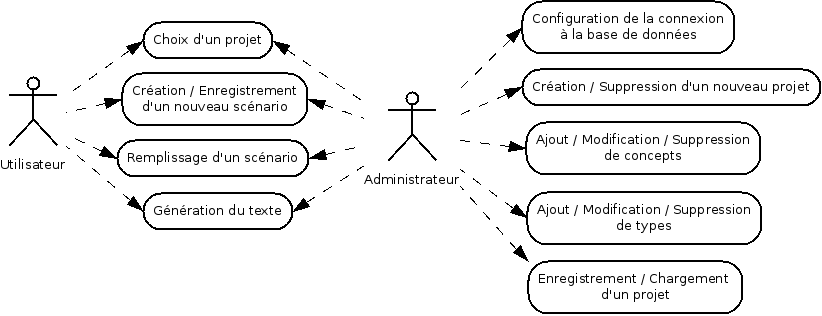
\includegraphics[scale=0.5]{cas_utilisation.png}

\subsection{Schémas de fonctionnement}

Ils schématisent les interactions entre le programme, l'utilisateur et l'administrateur, avec la base de données et Syntox.


Avant tout, l'administrateur configure la connexion avec la base de données.

Ensuite, il crée des types et concepts (ayant un nom, un type et des arguments) et qu'il associe avec ceux crée par analyse de la base de données: ces concepts sont primordiaux pour la production finale de texte et régissent la manière dont est interrogée la base de données.


%Il se doit de compléter la grammaire (s'il en existe une) et d'enrichir le lexique pour répondre aux concepts que l'on souhaite expliquer; autrement dit, chaque base de données aura besoin de son propre lexique et éventuellement d'un ajustement de la grammaire pour obtenir un résultat satisfaisant.

L'utilisateur peut alors sélectionner un scénario ou interroger la base de données avec les outils proposés par l'IHM. Ses actions vont donner aux programmes les paramètres nécessaires à la création d'une entrée Syntox, après la récupération des informations nécessaires via des requêtes SQL. Syntox est alors sollicité pour générer un texte final.

A l'heure actuelle, on ne sait pas encore si le résultat final sera consultable uniquement via Syntox ou renvoyé à l'utilisateur via notre logiciel.

	\subsubsection{Schéma de fonctionnement - Utilisateur}
	Le schéma suivant décrit le fonctionnement du logiciel du point de vue d'un utilisateur classique.
	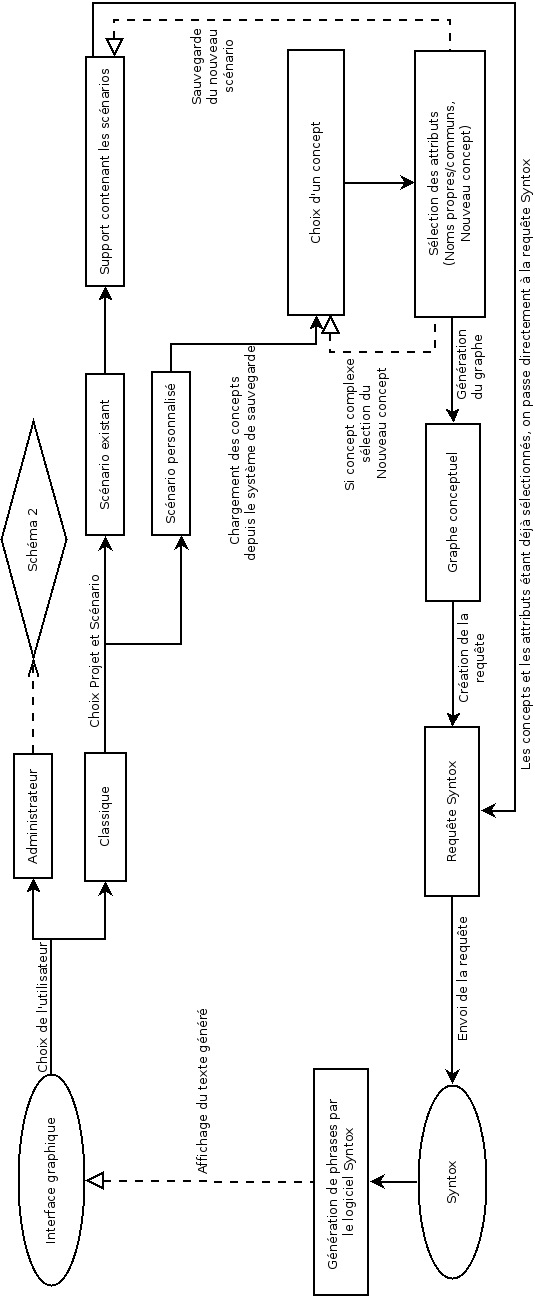
\includegraphics[scale=0.45]{FonctionnementUtilisateur.png}
	

	\subsubsection{Schéma de fonctionnement - Administrateur}
	Le schéma suivant décrit le fonctionnement du logiciel du point de vue d'un administrateur.
	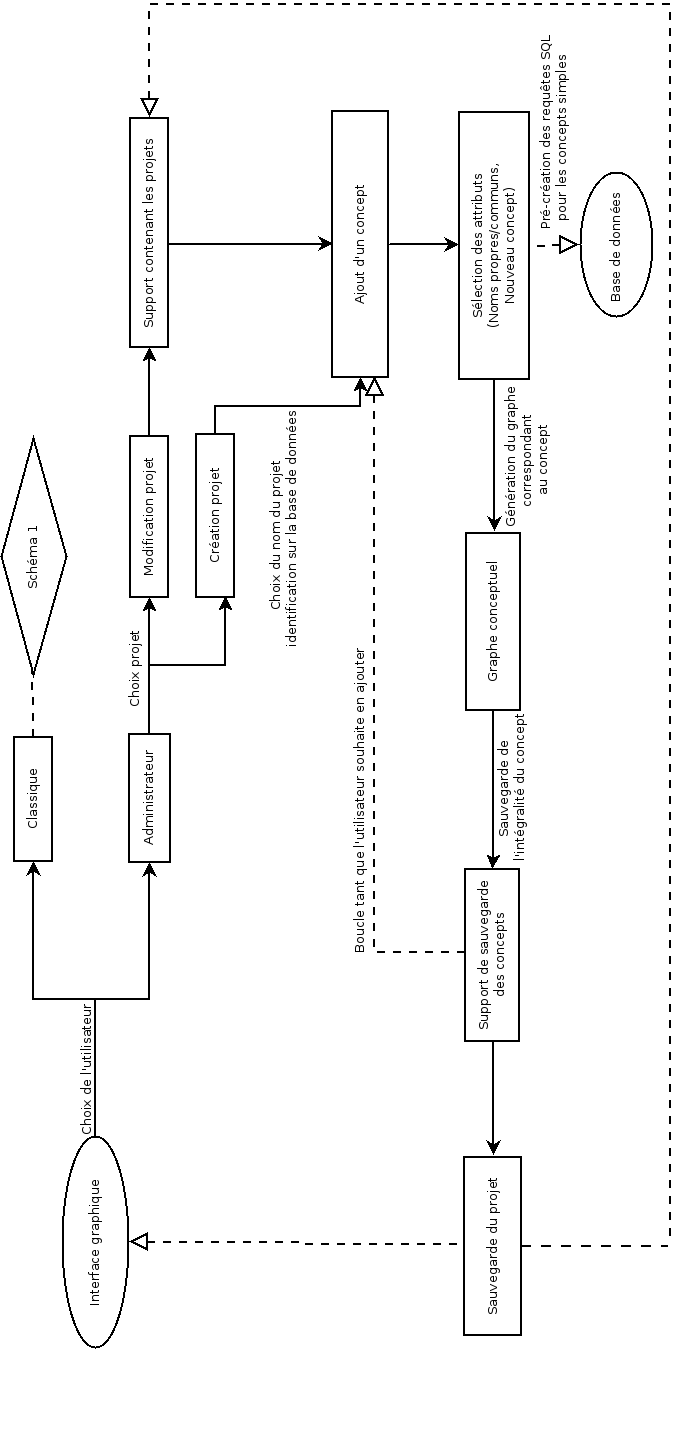
\includegraphics[scale=0.45]{FonctionnementAdministrateur.png}

	



\section{Diagramme de packages}
Le diagramme suivant présente la structure générale du logiciel.

\begin{center}
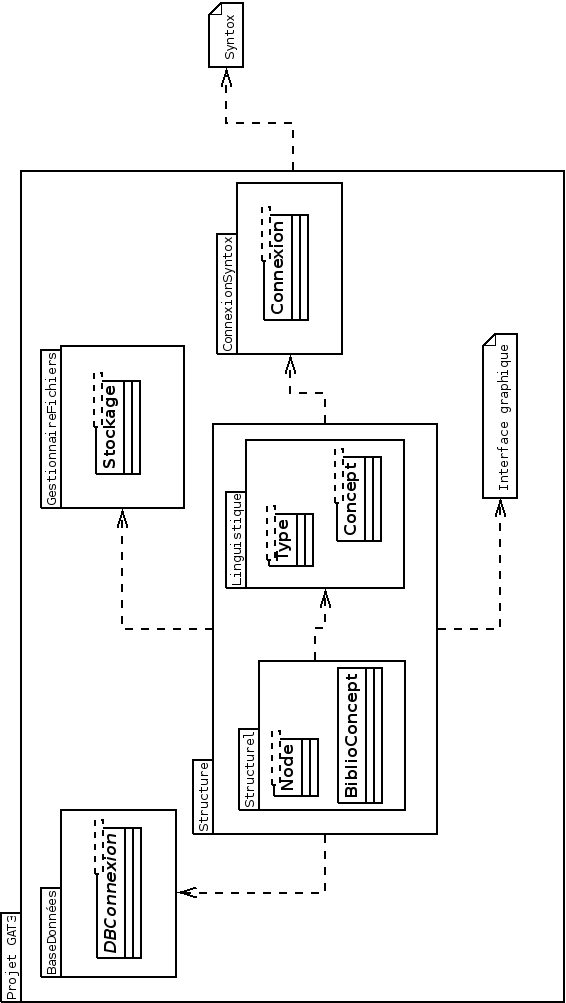
\includegraphics[scale=0.45]{DiagPackages.png}
\end{center}


Notre programme se composera de cinq packages principaux: Database, Linguistic, FileManager, SyntoxConnection et IHM, correspondant aux différentes fonctionnalités du programme.
Chacun de ces packages comportera les classes nécessaires à son bon fonctionnement.

% Expliquer le diagramme de packages





\section{Base de données}

\subsubsection*{Package databaseInspection}

\begin{itemize}
\item Interface Base: Cette interface sera implémentée par BaseImpl. Elle contient les tables et leurs relations(jointure).
\item Interface Table: Cette interface sera implémentée par TableImpl. Elle représente une table et contient les liste de ces colonnes.
\item Interface Column: Cette interface sera implémentée par ColumnImpl. Elle représente une colonne d'une table.
\item Interface JoinTable: Cette interface sera implémentée par JoinTableImpl. Elle représente la liaison entre deux table.
\item Interface BaseFactory: Cette interface sera implémentée par BaseFactoryImpl. elle construit un objet Base à partir d'une base de données SQL.
\item Interface RequestMaker: Cette interface sera implémentée par RequestMakerImpl. Elle construit une requête SQL.
\item Interface AgloTable: Cette interface sera implémentée par AgloTableImpl. Elle calcule la jointure minimal entre plusieurs table.
\end{itemize}

\begin{figure}[h!]
\begin{center}
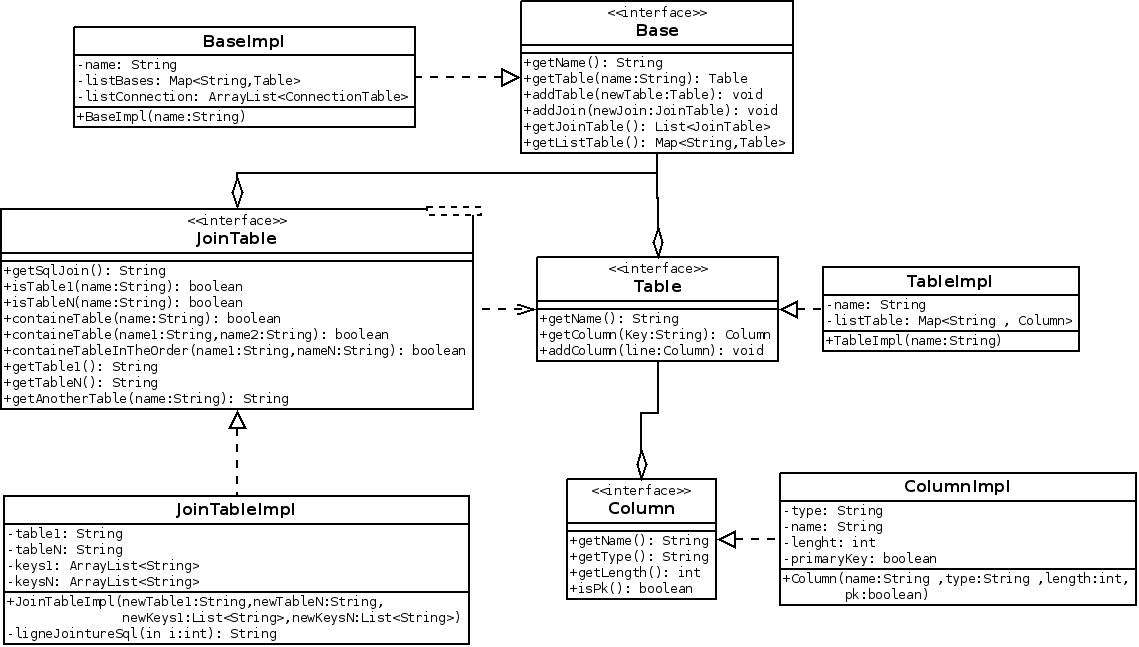
\includegraphics[scale=0.4]{bduml/structDataBase.png}
\caption{Diagramme du package databaseInspection partie structure}
\end{center}
\end{figure}

\begin{figure}[h!]
\begin{center}
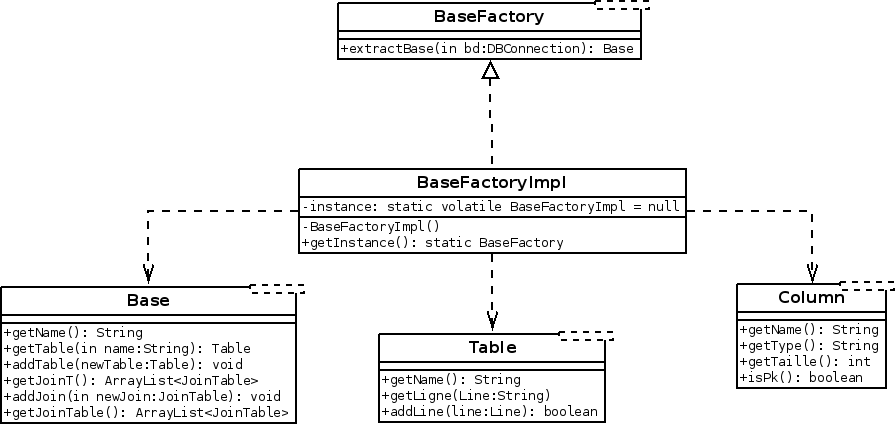
\includegraphics[scale=0.5]{bduml/baseFactory.png}
\caption{Diagramme du package databaseInspection partie génération de la structure}
\end{center}
\end{figure}

\begin{figure}[h!]
\begin{center}
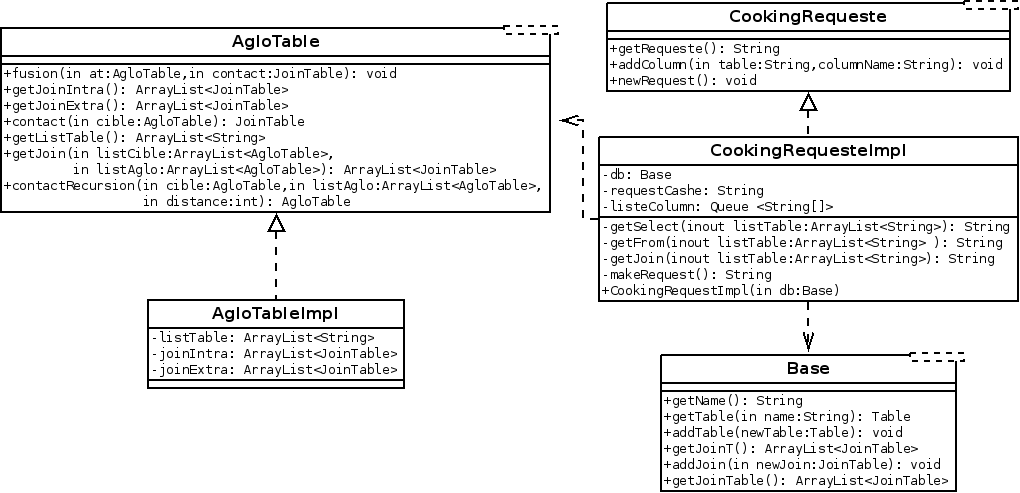
\includegraphics[scale=0.5]{bduml/cookingRequeste.png}
\caption{Diagramme du package databaseInspection partie génération de requête sql}
\end{center}
\end{figure}


\subsubsection*{Package databaseConnection}

\begin{center}
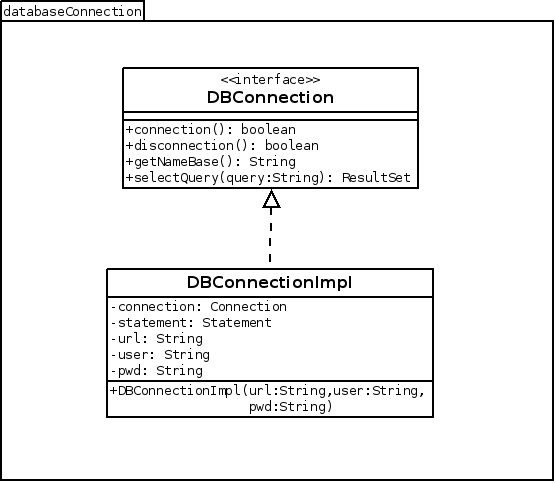
\includegraphics[scale=0.5]{bduml/databaseConnection.png}
\end{center}


\begin{itemize}
\item Interface DBConnexion: Cette interface sera implémentée par DBConnexionImpl. Elle contient les outils nécessaire à la connexion aux bases de données.
\end{itemize}



\section{Package Linguistic}

Ce package comprend toutes les classes nécessaires à la gestion des concepts, la mise en place d'un système de typage et la génération du graphe conceptuel correspondant au scénario généré par l'utilisateur.

Le package \texttt{linguistic} a été subdivisé en trois sous-packages : \texttt{concepts\_gestion}, \texttt{types\_gestion} et \texttt{graph\_concepts\_gestion}.

\begin{center}
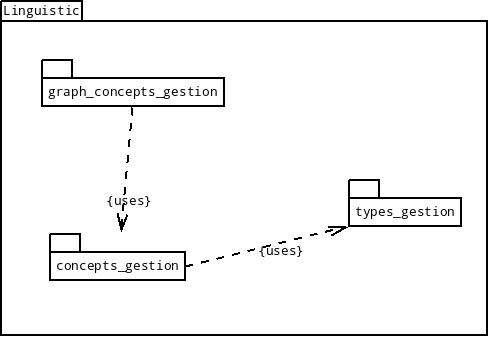
\includegraphics[scale=0.5]{DiagLinguisticPackages.png}
\end{center}

\subsection{Package \texttt{concepts\_gestion}}

\begin{center}
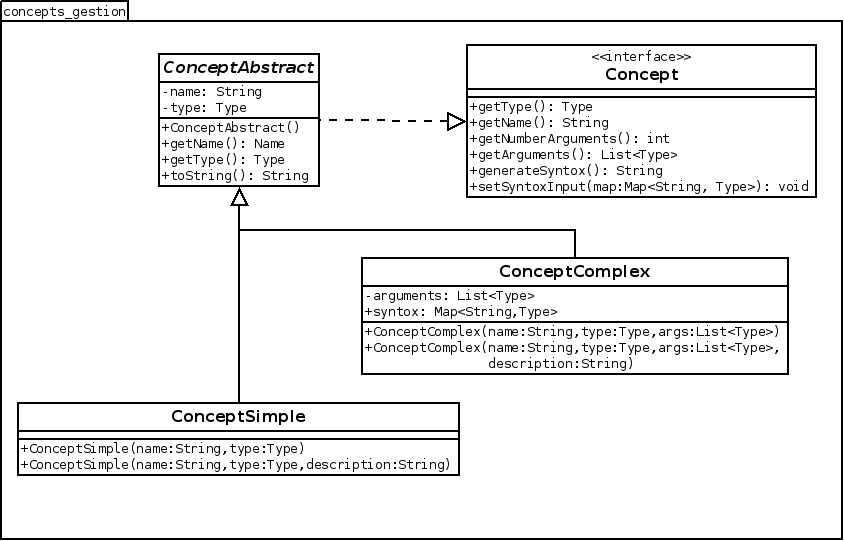
\includegraphics[scale=0.5]{DiagLinguistic_concepts_gestion.png}
\end{center}

Ce package contient la structure représentant un concept. Chaque \texttt{Concept} est défini par (au moins) un nom et un \texttt{Type}. Le \texttt{Concept} peut être simple ou complexe ; s'il est complexe, il possède également une liste d'arguments (qui sont des types, ce qui permet une indépendance des différents concepts). % voir parametre syntox et methode setSyntoxInput...

La classe \texttt{ConceptAbstract} permet de factoriser du code, notamment les accesseurs.
La méthode \emph{generateSyntox()} sera analysée dans la partie "Package Syntox".

\subsection{Package \texttt{types\_gestion}}

\begin{center}
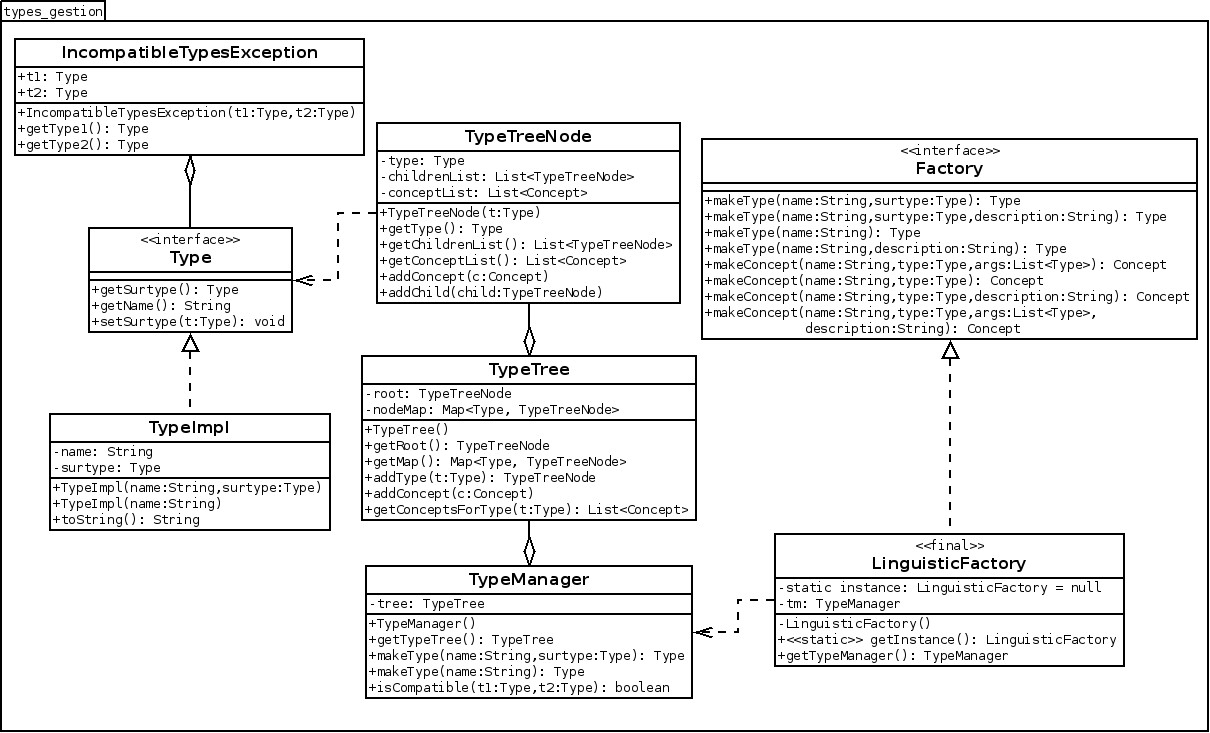
\includegraphics[scale=0.43]{DiagLinguistic_types_gestion.png}
\end{center}

Le package \texttt{types\_gestion} contient les classes gérant le système de typage des \texttt{Concept}. Le coeur de ce package est donc bien sûr l'interface \texttt{Type} et la classe \texttt{TypeImpl} qui l'implémente.
Chaque \texttt{Type} est défini par son nom et peut être relié à d'autres types par une relation surtype/sous-type.

\bigskip

Les \texttt{Type} sont stockés dans un arbre de types, implémenté par la classe \texttt{TypeTree}. Cet arbre de types contient une référence à la racine de l'arbre (qui correspond au Type racine), et une \texttt{Map} qui permet de faire la correspondance entre un \texttt{Type} stocké dans l'arbre et le noeud de l'arbre associé à ce \texttt{Type}. Nous avons choisi d'implémenter cette correspondance avec une \texttt{Map} car c'est une structure qui permet une indexation par les \texttt{Type}, et un accès rapide en lecture.

L'arbre de types \texttt{TypeTree} est composé de plusieurs \texttt{TypeTreeNode}, chacun correspondant à un \texttt{Type} précis et une liste de \texttt{Concept} ayant ce \texttt{Type}. Chaque \texttt{TypeTreeNode} comprend aussi une liste des \texttt{TypeTreeNode} qui sont "en-dessous" de lui dans l'arbre de types (et qui sont donc associés à ses "sous-types").

Cette connaissance par chaque \texttt{TypeTreeNode} de ses fils permet au \texttt{TypeTree} de parcourir les \texttt{TypeTreeNode} à partir de la racine, ce qui sert notamment pour l'implémentation de la méthode \emph{getConceptsForType(Type t)}, qui retourne une liste des instances de \texttt{Concept} ayant le \texttt{Type} \emph{t} ou un de ses sous-types.

\bigskip

La classe \texttt{TypeManager} est une classe qui permet de gérer la classe \texttt{TypeTree} et d'instancier la classe \texttt{TypeImpl}, elle se base sur le modèle du pattern Factory. En effet, l'instanciation de \texttt{TypeImpl} est faite par le \texttt{TypeManager}, qui crée et modifie dynamiquement l'arbre de types correspondant. Il est aussi responsable de la compatibilité de deux \texttt{Type} \emph{t1} et \emph{t2}, c'est-à-dire la vérification que le \texttt{Type} \emph{t1} est un sous-type (strict ou non) du \texttt{Type} \emph{t2}.

\bigskip

L'arbre de types et donc la classe \texttt{TypeManager} ne doivent avoir qu'une seule instance par \texttt{Projet}, nous avons donc mis en place la classe \texttt{LinguisticFactory}, qui se base sur le pattern Singleton, pour gérer la création de nouveaux \texttt{Type} et de nouveaux \texttt{Concept}. C'est cette classe qui sera utilisée lors de l'instanciation des \texttt{Type} et des \texttt{Concept}, et qui "cachera" à l'utilisateur le système de gestion et de stockage des \texttt{Type} et des \texttt{Concept}.

\bigskip

Le package \texttt{types\_gestion} comprend également une classe d'exception \texttt{IncompatibleTypesException}, qui permet de gérer l'incompatibilité de deux types.

\subsection{Package \texttt{graph\_concepts\_gestion}}

\begin{center}
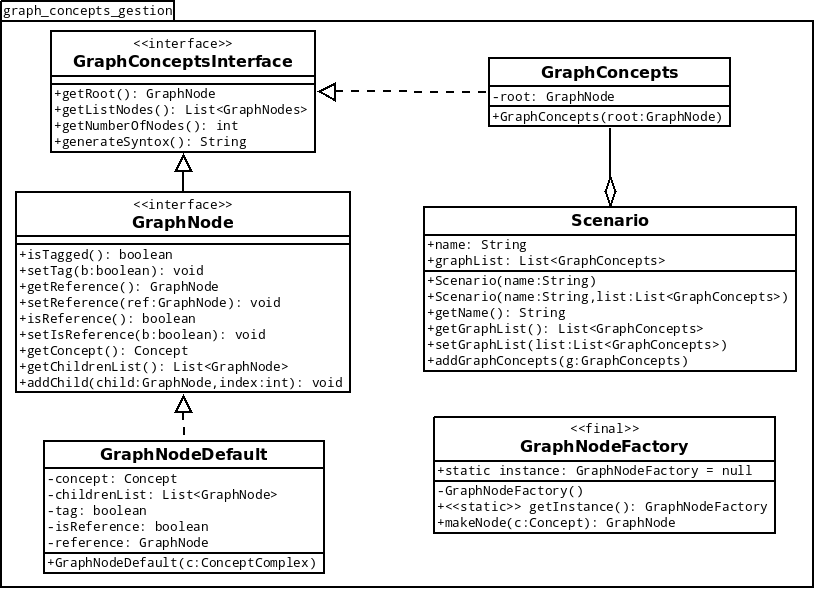
\includegraphics[scale=0.5]{DiagLinguistic_graph_concepts_gestion.png}
\end{center}

A la fin de la création et du remplissage d'un nouveau scénario, les \texttt{Concept} manipulés par l'utilisateur sont stockés dans un graphe, implémenté à l'aide des classes \texttt{GraphNodeDefault} et \texttt{GraphConcepts}, et des interfaces \texttt{GraphConceptsInterface} et \texttt{GraphNode}.

Chaque \texttt{GraphConcepts} est constitué d'un \texttt{GraphNode} racine. Un \texttt{GraphNode} est identifié par le \texttt{Concept} qu'il représente et la liste des \texttt{GraphNode} dont il est le "parent".

\bigskip

Par construction, le graphe créé à partir des \texttt{Concept} manipulés par l'utilisateur est un graphe orienté acyclique (l'orientation se fait d'un \texttt{GraphNode} vers ses "fils", dont il possède la liste). Cependant, ce graphe doit être enregistré dans un fichier XML et il était plus simple pour cette utilisation d'avoir une structure purement arborescente. 

Nous avons donc ajouté trois champs qui nous permettent d'avoir une structure d'arbre tout en conservant la possibilité d'avoir des références multiples à un même concept ; ces champs sont principalement utilisés dans la méthode \emph{addChild(GraphNode child, int index)} de la classe \texttt{GraphNodeDefault}.
\begin{itemize}
\item \emph{tag} (\texttt{boolean}) : ce champ est modifié lors du parcours de la liste de \texttt{GraphNode} \emph{childrenList}, il permet de savoir si le \texttt{GraphNode} que l'on veut ajouter a déjà été rencontré parmi les enfants du \texttt{GraphNode} considéré. Si cela est le cas, cela signifie que l'on va avoir une référence multiple au même \texttt{GraphNode}, et donc au même \texttt{Concept}.
\item \emph{isReference} (\texttt{boolean}) : ce champ a pour valeur \emph{true} si d'autres \texttt{GraphNode} font référence au \texttt{GraphNode} considéré.
\item \emph{reference} (\texttt{GraphNode}) : ce champ contient le \texttt{GraphNode} auquel on fait référence, le cas échéant.
\end{itemize}

On a donc un arbre de \texttt{GraphNode} au lieu d'un graphe acyclique ; si deux \texttt{GraphNode} ayant trait au même \texttt{Concept} sont présents dans cet arbre, alors c'est que l'un fait référence à l'autre.

\bigskip 
Les scénarios (qui seront plus tard enregistrés dans un fichier .XML) sont représentés par un nom et une liste de \texttt{GraphConcepts}.

\bigskip
Le pattern Singleton est ici réutilisé comme modèle pour la classe \texttt{GraphNodeFactory}, qui permet d'instancier la classe \texttt{GraphNodeDefault} en cachant l'implémentation du graphe de \texttt{Concept}.

\section{Package Syntox}
 
\begin{center}
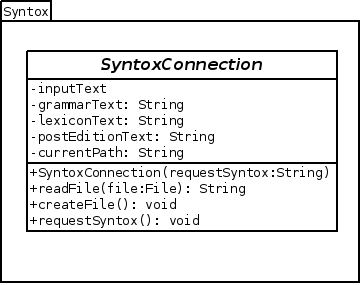
\includegraphics[scale=0.6]{diversuml/SyntoxConnection.png}
\end{center}

Ce package contient les éléments permettant de communiquer avec le module Syntox accessible depuis internet. Le package Syntox comporte les éléments suivants : une classe SyntoxConnection, grammar.txt, lexicon.txt, postEdition.txt, headerPage.html et endingPage.html.

\bigskip
La classe SyntoxConnection permet de coordonner les éléments présents dans le package afin de concevoir une page HTML, pdp.html, permettant d'établir la communication avec Syntox. Elle reçoit en entrée la requête Syntox au préalable formater par la méthode generateSyntox() des classes GraphConcepts et GraphNodeDefault du package linguistic. 

\bigskip
Les fichiers .txt comportent les autres éléments que le logiciel Syntox à besoin de posséder pour la génération du texte mais dont nous ne devons pas nous charger de générer. Parmi ces éléments nous avons la grammaire qui est stockée dans grammar.txt, le lexique dans le fichier lexicon.txt, et enfin les outils syntaxiques supplémentaires dans postEdition.txt. 

\bigskip
De la même façon, les fichiers headerPage.html et endingPage.html contiennent les éléments nécessaires à la page HTML. C'est à dire l'entête de la page, qui comporte entre autre le descriptif de la page, l'ouverture du formulaire ainsi que la requête Syntox, et en bas de page, qui quant à elle contient les balises de fermetures du formulaire et du corps de la page. 

\bigskip
L'utilisation de la méthode requestSyntox() de la classe SyntoxConnection permet la construction de la page HTML ainsi que le lancement automatique de cette dernière dans le navigateur par default de l'utilisateur. Cette méthode fait appel dans un premier temps à createFile() une méthode qui va assembler chaque éléments nécessaires dans le fichier pdp.html. Nous avons dans un premier temps l'écriture de l'entête de la page HTML, headerPage.html. La requête Syntox, contenu dans la variable inputText, est directement insérée à la suite. Puis respectivement le contenu des fichiers grammar.txt, lexicon.txt et postEdition.txt est ajouté afin de constituer le corps de la page. Pour finir, le contenu de endingPage.html est à son tour recopié pour clôturer la création de la page. 

\bigskip
Blablabla    


\section{Gestion des fichiers}


\begin{center}
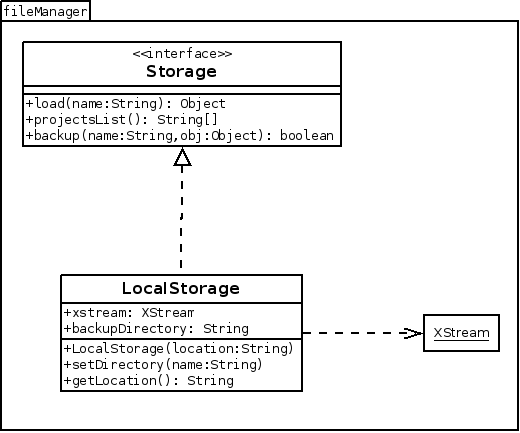
\includegraphics[scale=0.55]{diversuml/fileManager.png}
\end{center}


\subsection{Présentation globale}

	Dans le cadre de notre programme, il est indispensable de pouvoir à tout moment enregistrer le travail en cours sur
le disque dur et de pouvoir y accéder pour le modifier: en effet, les projets, scénarios et concepts doivent être modulables
et surtout, du fait de leur structure complexe, nécessitent un travail conséquent de la part de l'utilisateur, qui appréciera
de ne pas avoir besoin de recommencer son travail à chaque démarrage du programme.

	L'objet "Projet" regroupe tous les champs nécessaires au travail sur une base de donnée précise: scénarios, concepts et LinguisticFactory.
Il a donc été décidé que chaque Projet serait stocké sur le disque sous forme d'un fichier regroupant tous ses champs.

	Afin de faciliter la sérialisation des données, nous avons choisi d'utiliser la bibliothèque XStream.
Cette bibliothèque permet d'exporter facilement les objets sur le disque dur sous forme de fichier XML, et de les charger de manière également
intuitive.

	Pour cela nous avons ajouté la bibliothèque simplifiée "xstream-1.4.4.jar", qui regroupe les fonctions principales dont nous
aurons besoin afin de stocker et récupérer les objets de type Projet.

\subsection{Implémentation}

	Les fonctions nécessaires pour le chargement et enregistrement des données sont regroupées dans le package "fileManager".
Ce paquet contient l'interface Storage.java et son implémentation LocalStorage.java.

	Nous avons choisi d'implémenter cette partie de la manière suivante:
	\begin{itemize}
	\item Une fonction de chargement : public Object load (String name)
	\item Une fonction d'enregistrement : public boolean backup(String name, Object obj)
	\item Une fonction d'affichage des fichiers XML du répertoire courant : public String[] projectsList()
	\end{itemize}


Par défaut, on considère que le répertoire contenant les projets existants et stockant les nouvelles sauvegarde sera (en chemin relatif par rapport
au répertoire du programme): ../Projets

	\paragraph{Enregistrement}

La bibliothèque XStream permet donc l'enregistrement d'Objects sur le disque. Cette fonction se contente de créer un FileWriter du nom du paramètre "name"
à l'emplacement ../Projets et d'appeler la fonction xstream.toXML sur l'argument de type "Object"(on doit donc effectuer un cast sur le Project): on obtient un fichier .XML dans le répertoire contenant
toutes les informations nécessaire au travail sur le projet: les concepts existants, les scénarios déjà créés, et tous les types.

	\paragraph{Chargement}

La fonction "load" appelle simplement la fonction xstream.fromXML sur un fichier dont le nom est passé en paramètre de la fonction, et renvoie un Object,
que l'on cast en Project et qui peut être ensuite utilisé et modifié dans le programme.

	\paragraph{Affichage du répertoire courant}

Cette fonction renvoie un tableau de String dont les éléments sont les noms de fichiers .XML contenus dans le répertoire ../Projets, sans l'extension
de fichier. Cette fonction est utilisée dans la partie utilisateur du programme, au moment de choisir un projet existant.


	\paragraph{Utilisation des fonctions de chargement et d'enregistrement}

De part la manière de sauvegarder choisie, chaque modification (que ce soit un concept, un scénario ou un projet intégral) nécessite de sauvegarder
l'intégralité du projet: toutes les fonctions de sauvegarde du programme appellent la fonction backup de la classe LocalStorage après avoir modifié
l'objet chargé dans le programme.

On garantit ainsi l'intégrité du travail en cours par l'utilisateur au détriment éventuel du temps d'exécution: cependant, cette solution a été
préférée pour sa simplicité d'utilisation (une seule fonction de sauvegarde), pour sa propreté (un seul et unique fichier par projet, et non par scénario ou concept).

De plus, les structures de données utilisées, même si non limitées en taille par l'implémentation, ne seront de manière intuitive jamais gigantesques:
on ne peut pas imaginer une base de données associée à plusieurs millions de concepts ou de scénarios. Les temps d'éxécution des fonctions d'enregistrement
et de chargement sont donc considérées comme triviaux.

La fonction d'enregistrement est donc appelée à chaque clic sur un bouton de type "Enregistrer" (panel Scénario, Projet et Concept, administrateur ou utilisateur).
La fonction de chargement est utilisée lors du choix du projet existant par l'administrateur ou l'utilisateur (au lancement du programme dans la plupart des cas,
si l'utilisateur ne quitte pas le projet en cours pour en changer).
La fonction d'affichage du répertoire, quand à elle, est appelée au choix du projet, juste avant le chargement.


\section{Core}


\begin{center}
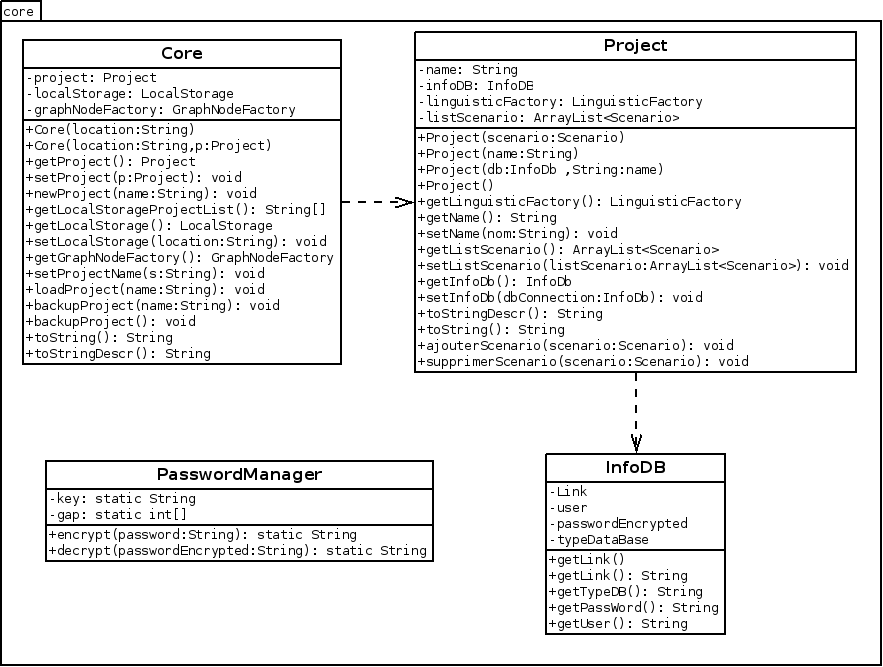
\includegraphics[scale=0.5]{diversuml/Core.png}
\end{center}

\section{Diagrammes de séquence}
	Ce diagramme de séquence explicite les étapes de configuration de la base de données, du lexique et de la grammaire par l'administrateur. 

	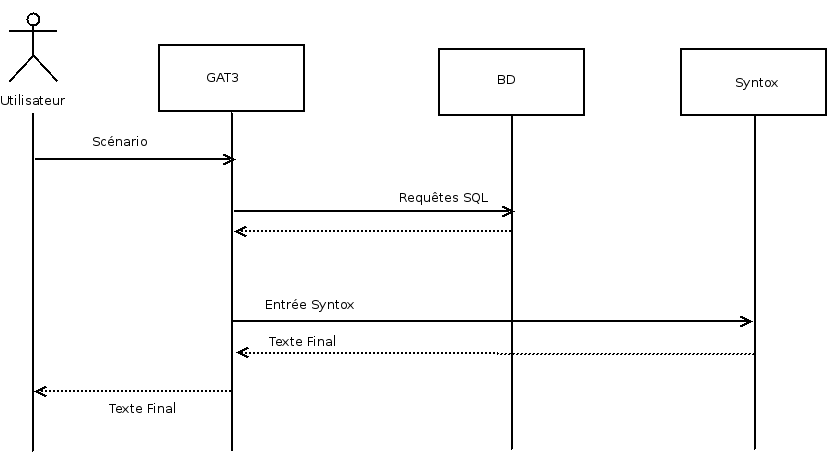
\includegraphics[scale=0.4]{diasequence2.png}

\begin{figure}[h!]
\begin{center}
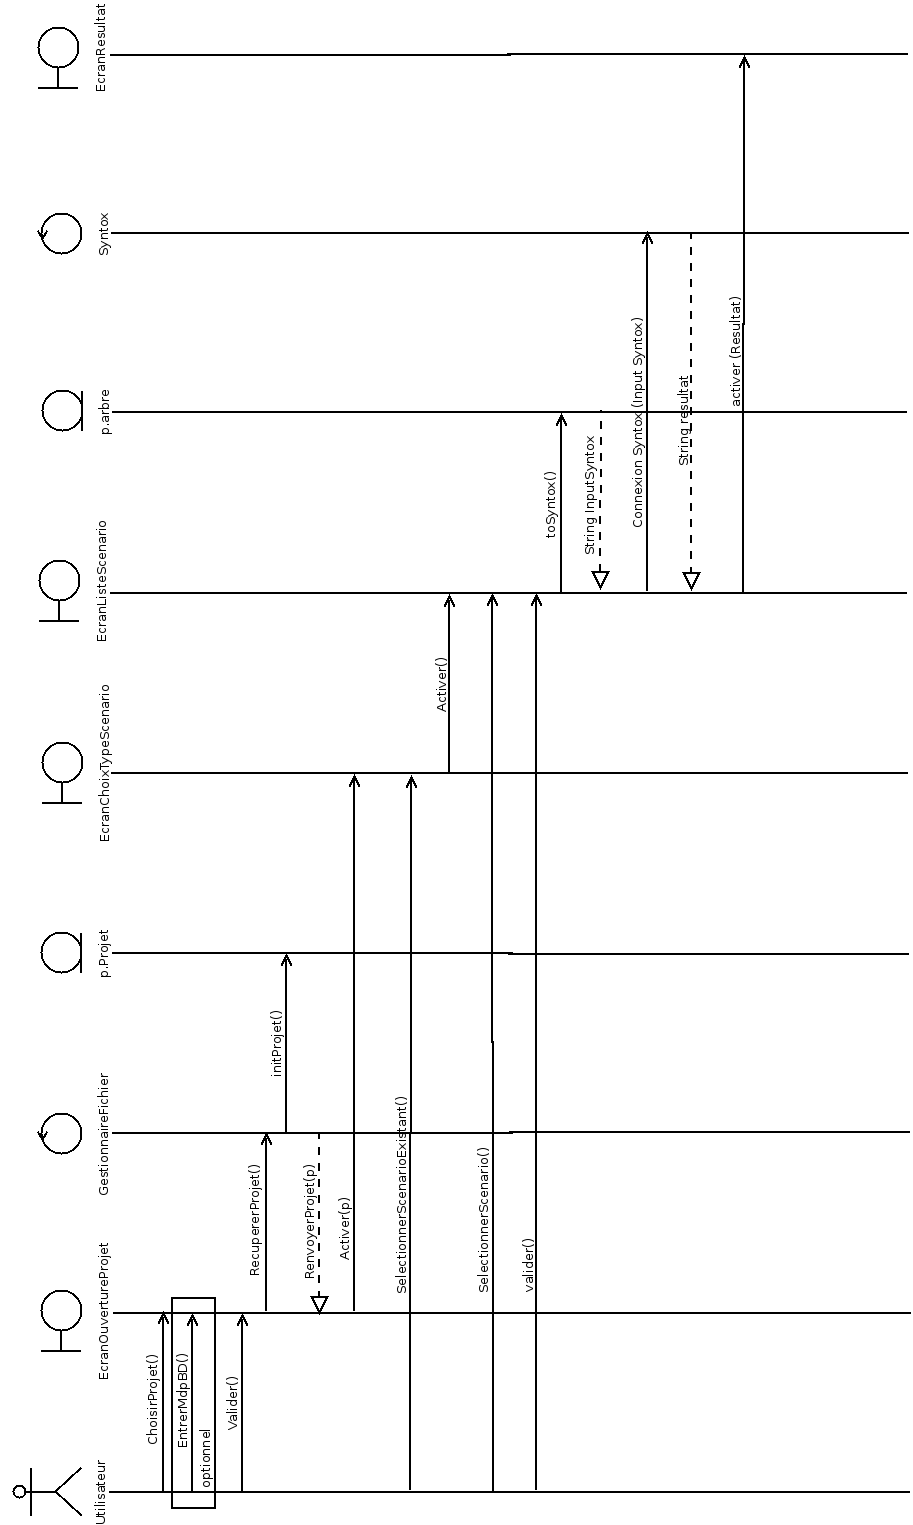
\includegraphics[scale=0.34]{DiagSeq.png}
\caption{Diagramme de séquence Scénario 1}
\end{center}
\end{figure}


\begin{figure}[h!]
\begin{center}
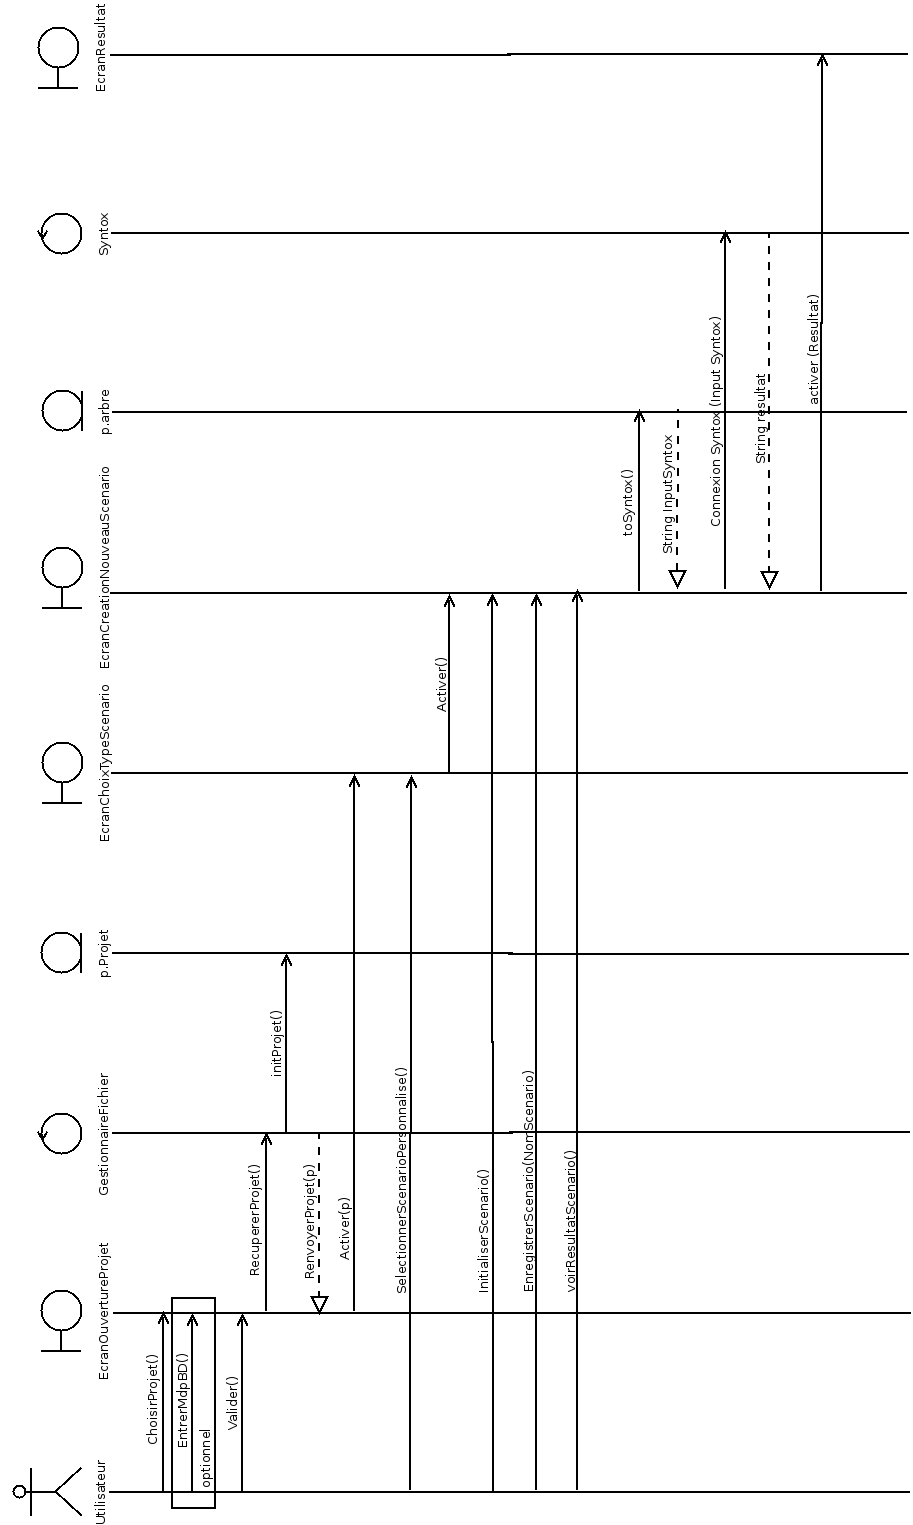
\includegraphics[scale=0.34]{DiagSeq2.png}
\caption{Diagramme de séquence Scénario 2}
\end{center}
\end{figure}


\begin{figure}[h!]
\begin{center}
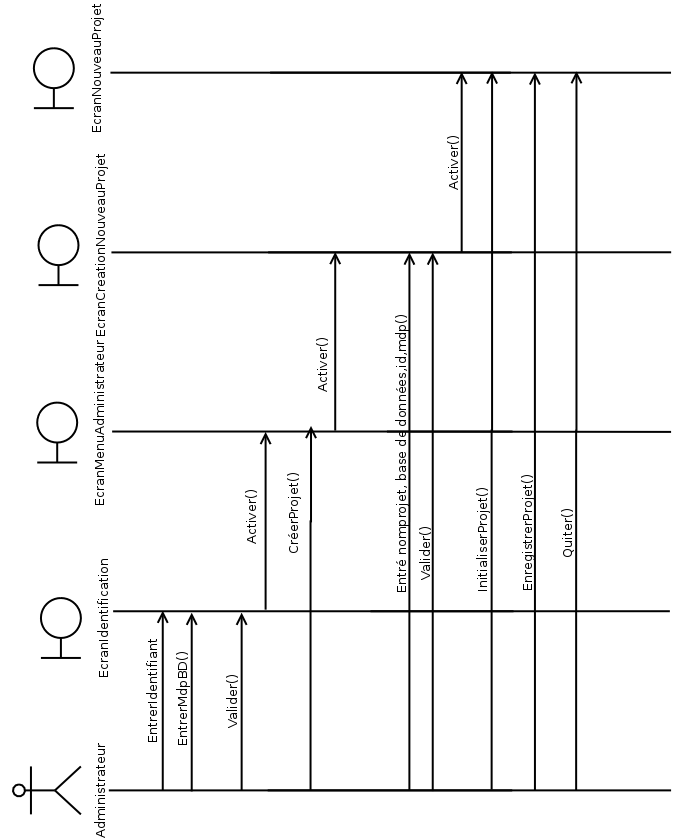
\includegraphics[scale=0.34]{DiagSeq3.png}
\caption{Diagramme de séquence Scénario 3}
\end{center}
\end{figure}


\chapter{Présentation du logiciel fourni}

% Explications et présentation de l'IHM
\begin{figure}
\centering
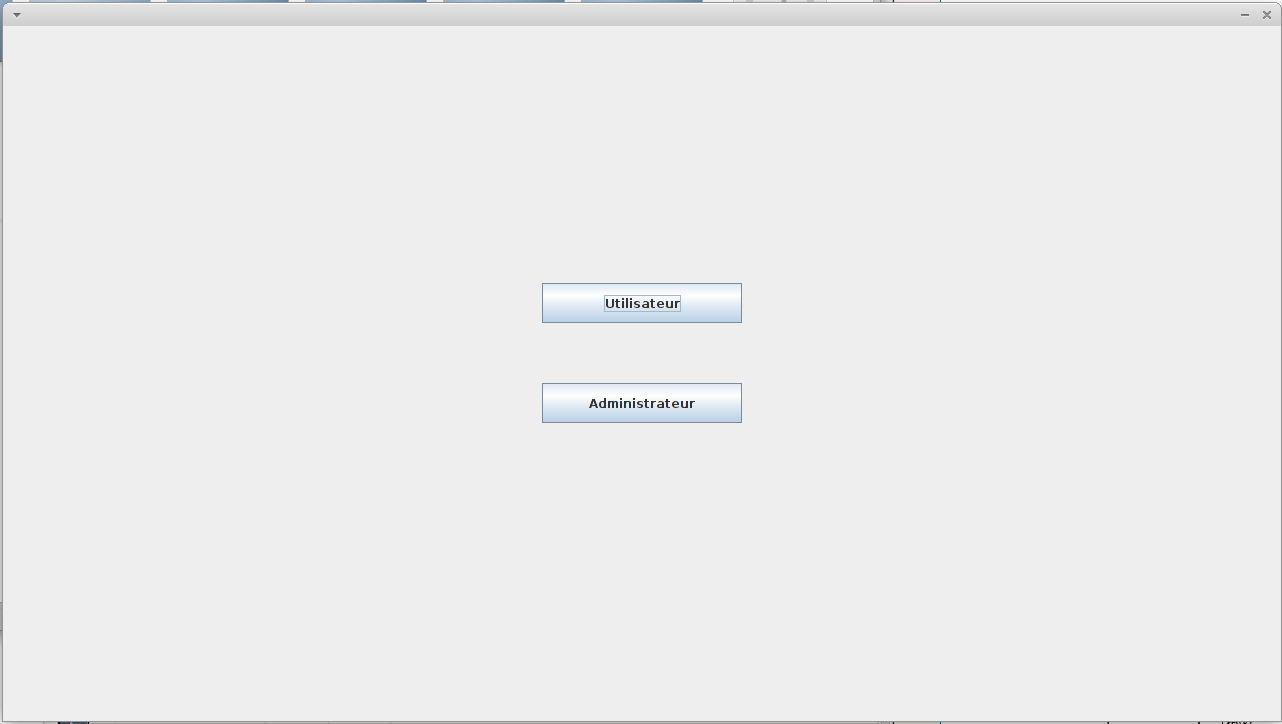
\includegraphics[scale=0.3]{IHM/accueil.png}
\caption{Ecran de connexion}
\end{figure}

\begin{figure}
\centering
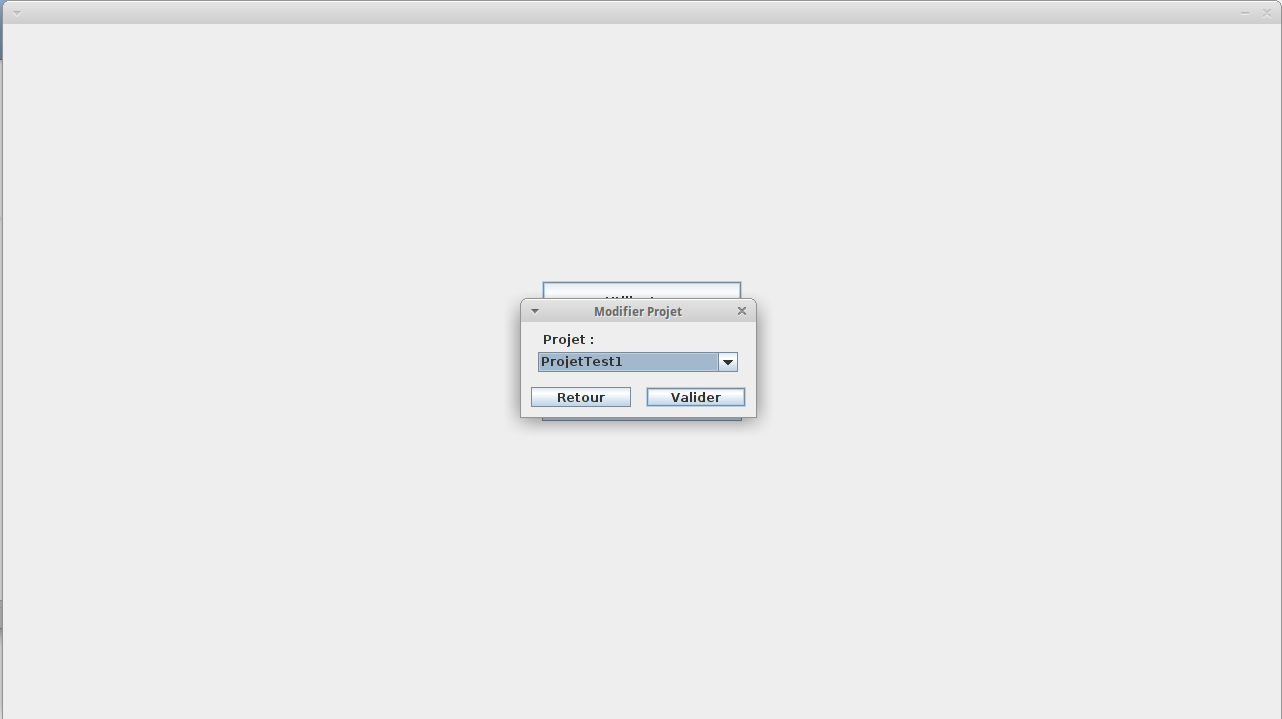
\includegraphics[scale=0.3]{IHM/selection_modifier_projet.png}
\caption{Ecran d'ouverture d'un projet}
\end{figure}

\begin{figure}
\centering
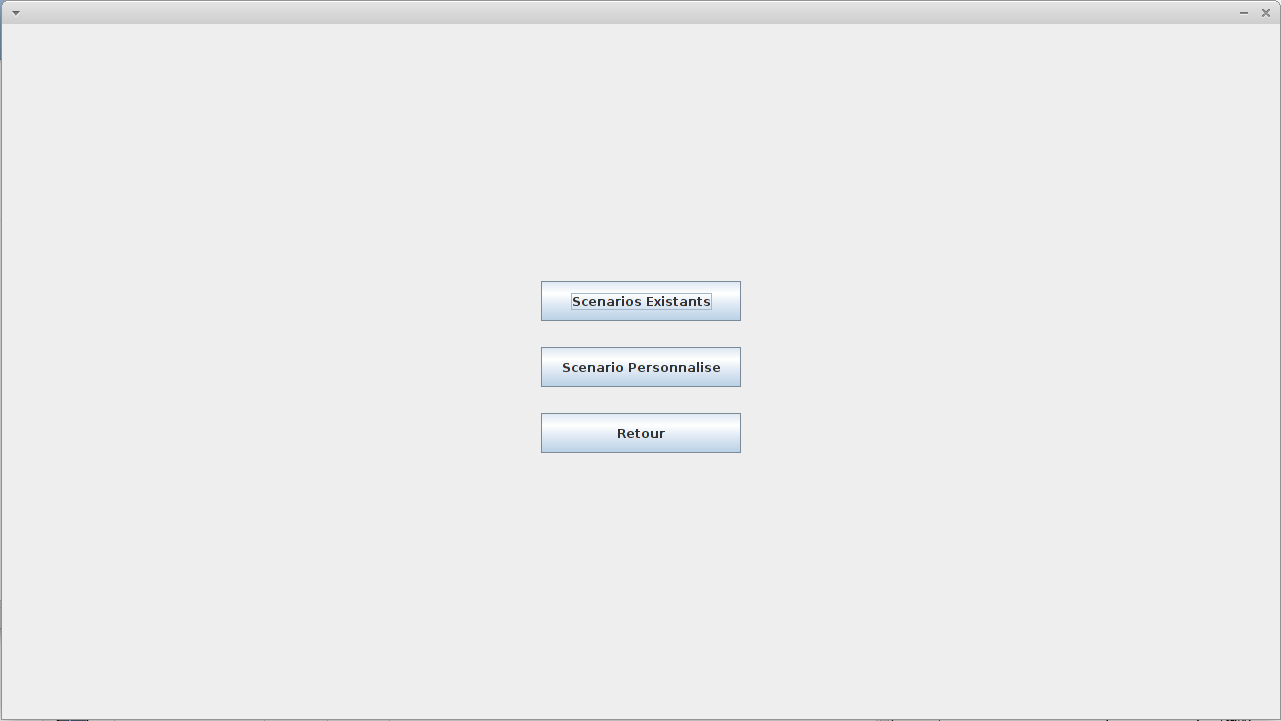
\includegraphics[scale=0.3]{IHM/choix_scenario.png}
\caption{Ecran de sélection de scénario existant/personnalisé}
\end{figure}
\begin{figure}
\centering
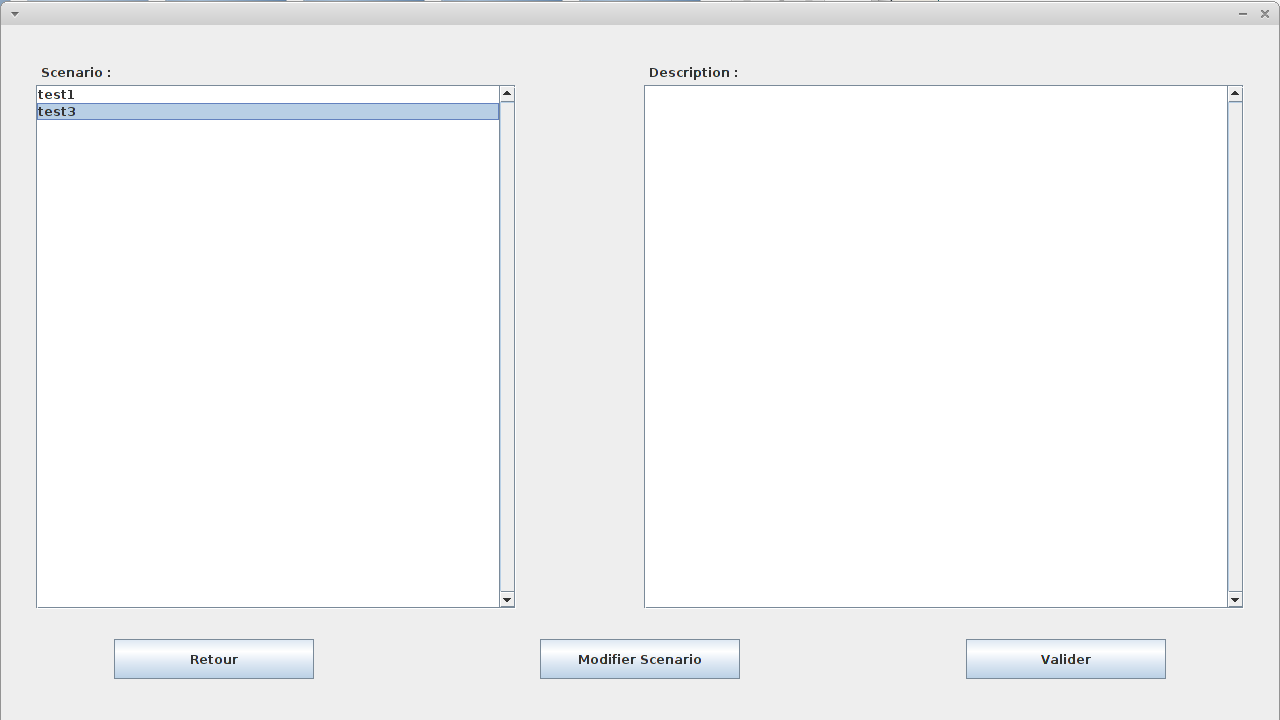
\includegraphics[scale=0.3]{IHM/selection_scenario.png}
\caption{Ecran de sélection de scénario existant}
\end{figure}
\begin{figure}
\centering
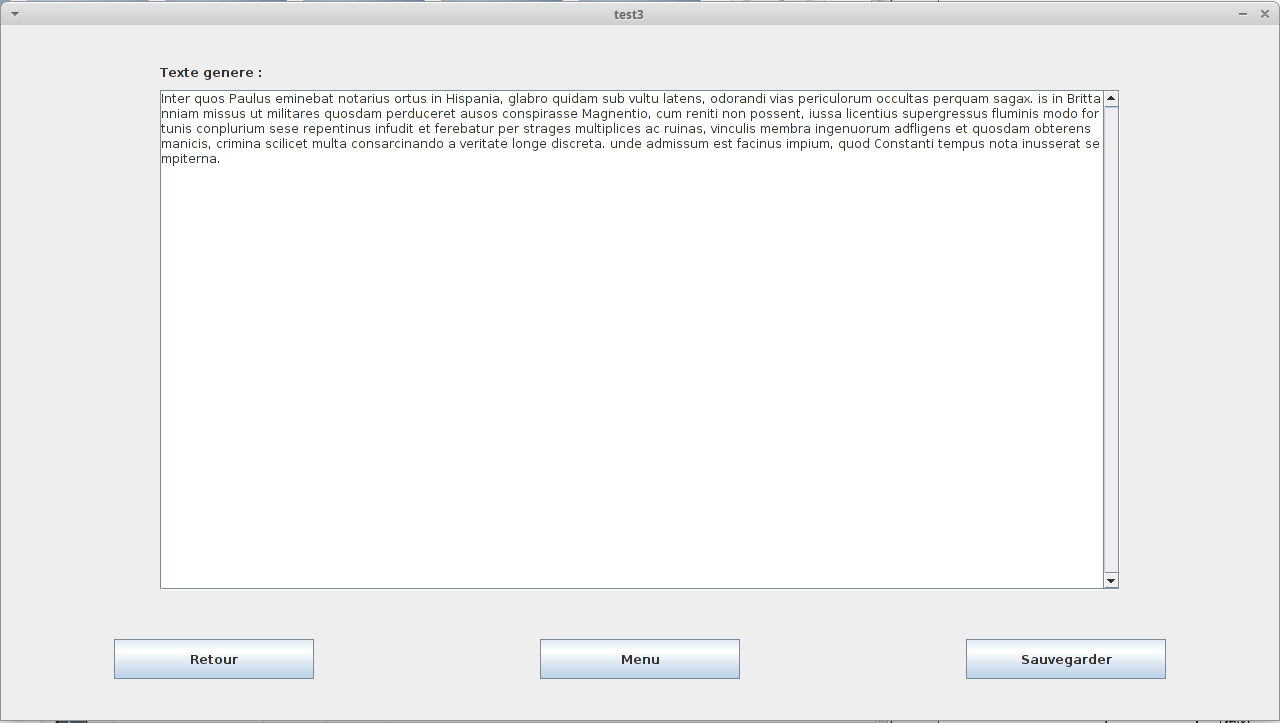
\includegraphics[scale=0.3]{IHM/affichage_resultat.png}
\caption{Ecran affichant le texte généré}
\end{figure}
\begin{figure}
\centering
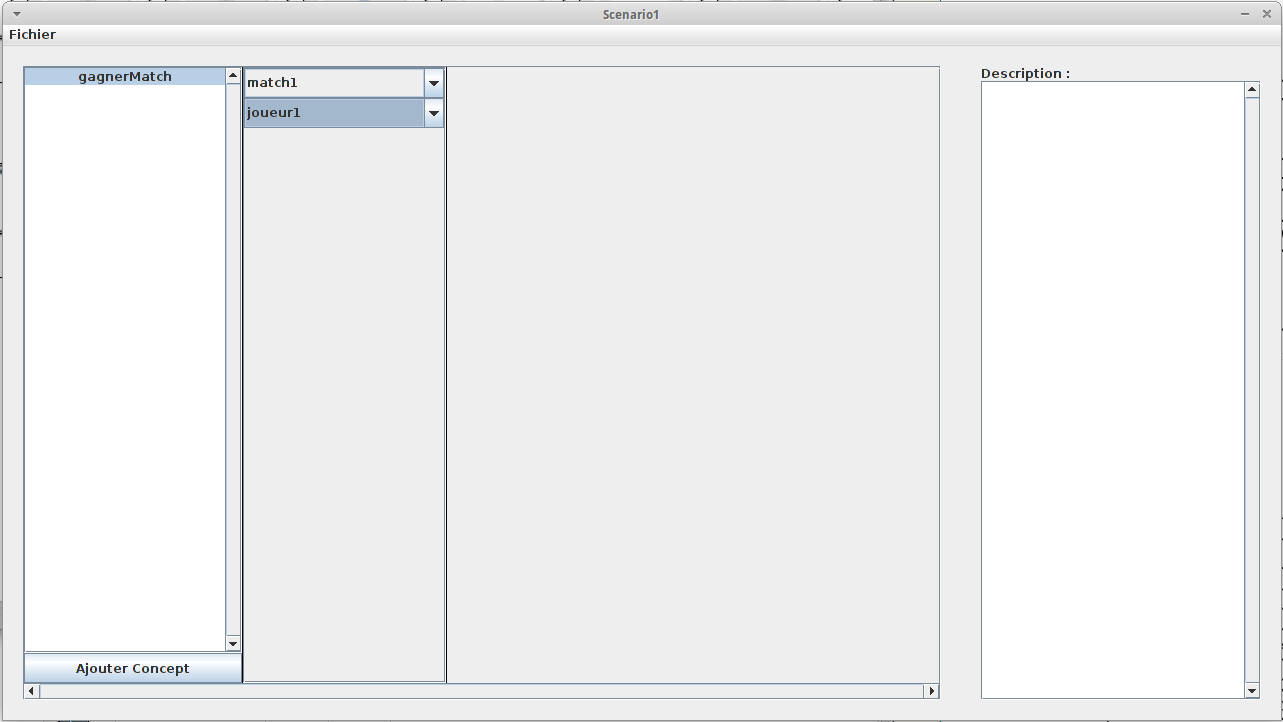
\includegraphics[scale=0.3]{IHM/remplissage_scenario.png}
\caption{Ecran de création d'un nouveau scénario}
\end{figure}
\begin{figure}
\centering
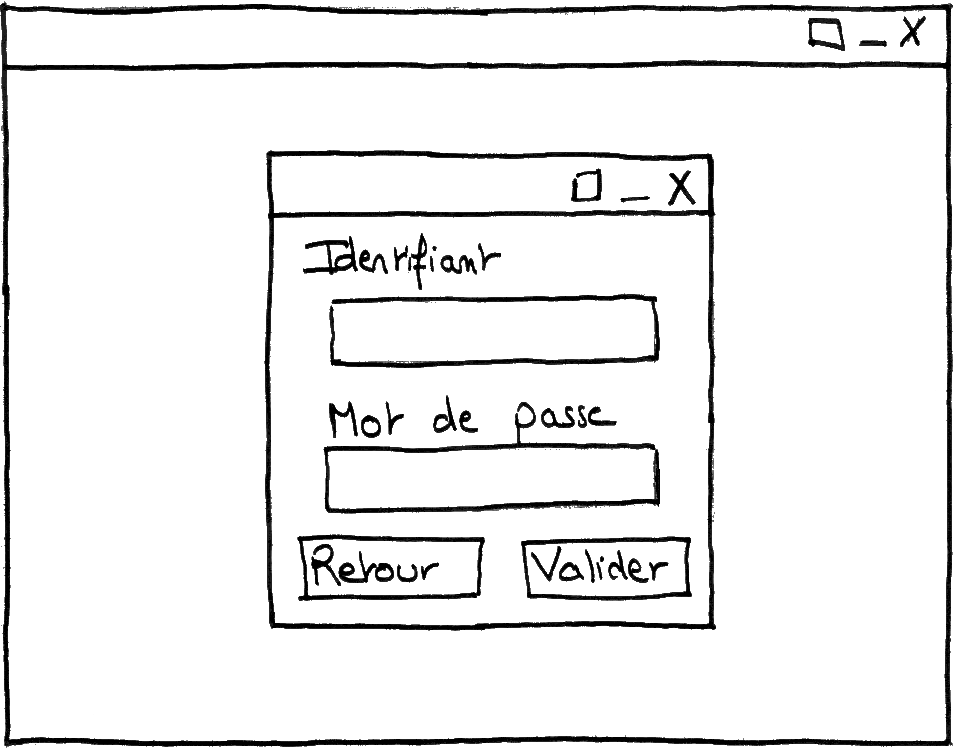
\includegraphics[scale=0.5]{IHM_5b.png}
\caption{Ecran de connexion à la partie administrateur}
\end{figure}
\begin{figure}
\centering
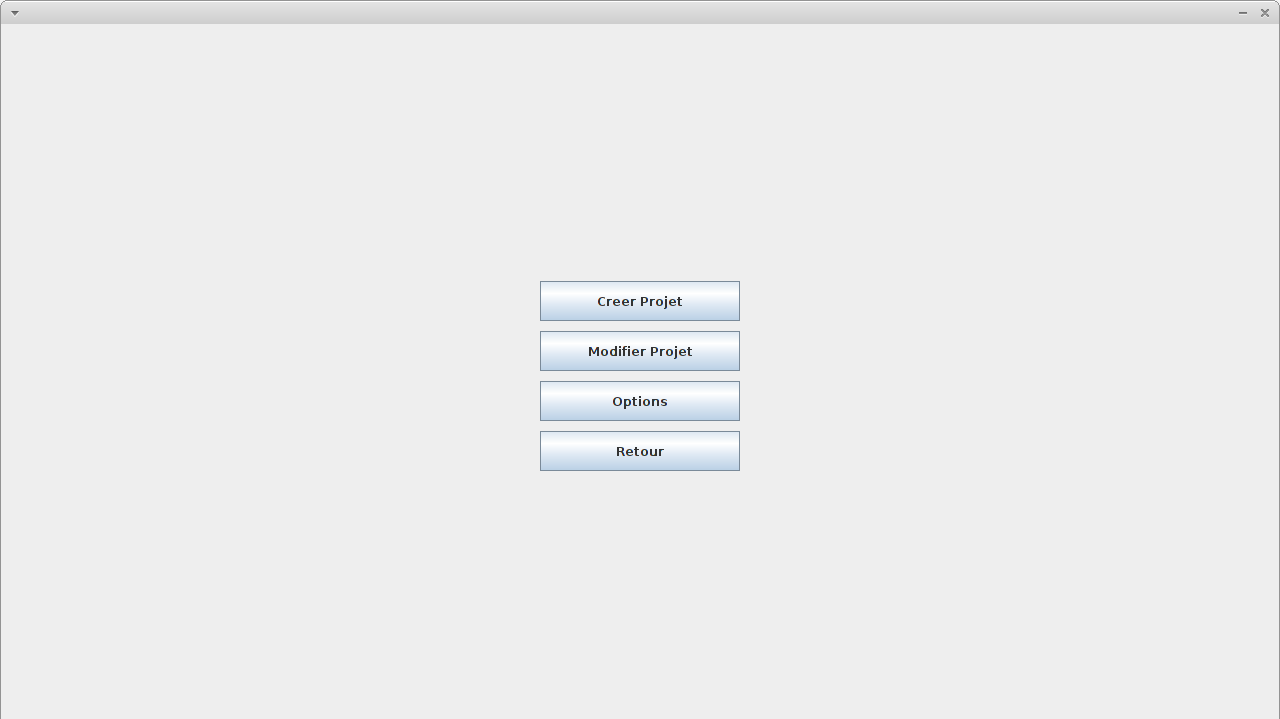
\includegraphics[scale=0.3]{IHM/selection_projet.png}
\caption{Ecran du menu administrateur}
\end{figure}
\begin{figure}
\centering
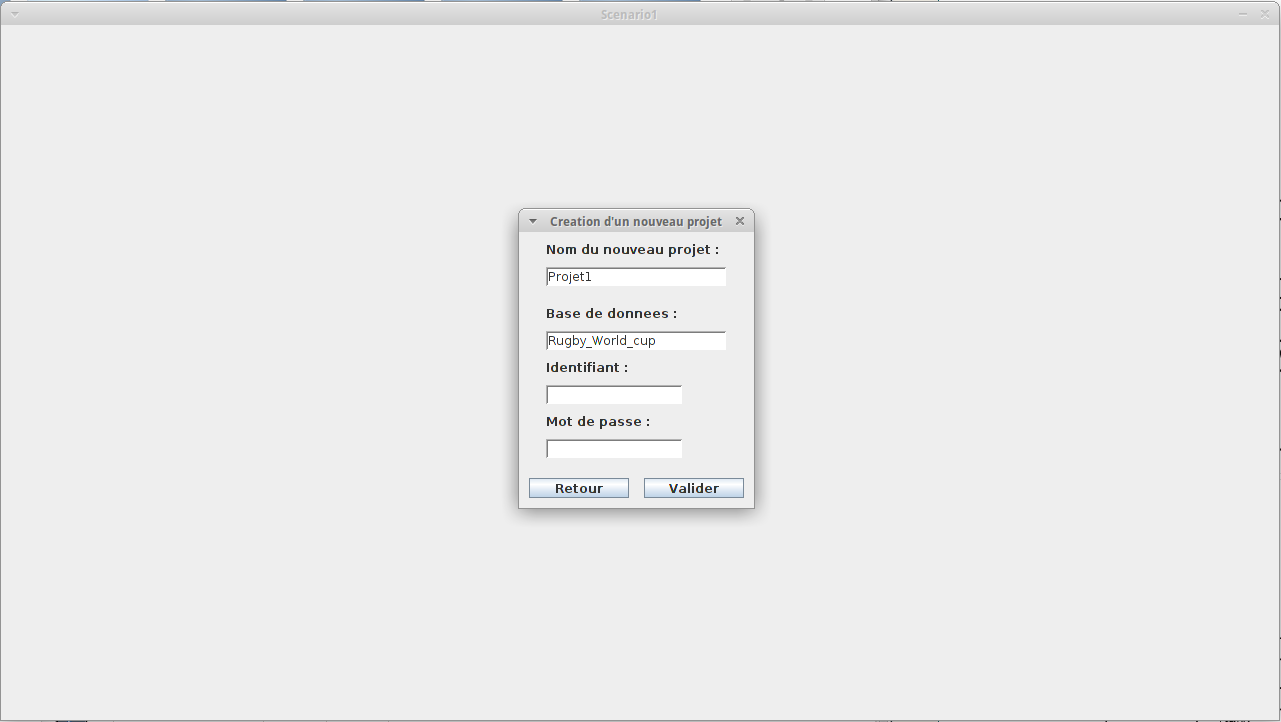
\includegraphics[scale=0.3]{IHM/creation_projet.png}
\caption{Ecran de création d'un nouveau projet}
\end{figure}
\begin{figure}
\centering
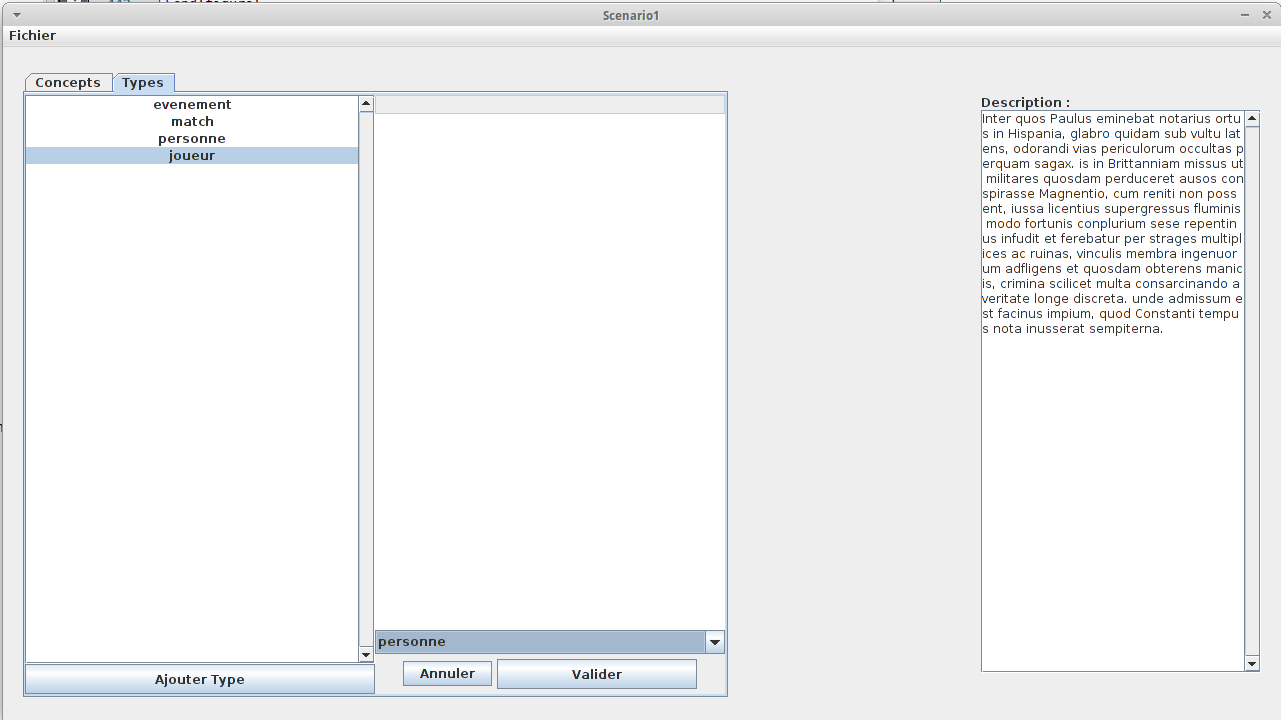
\includegraphics[scale=0.3]{IHM/creation_types.png}
\caption{Ecran de création des types}
\end{figure}
\begin{figure}
\centering
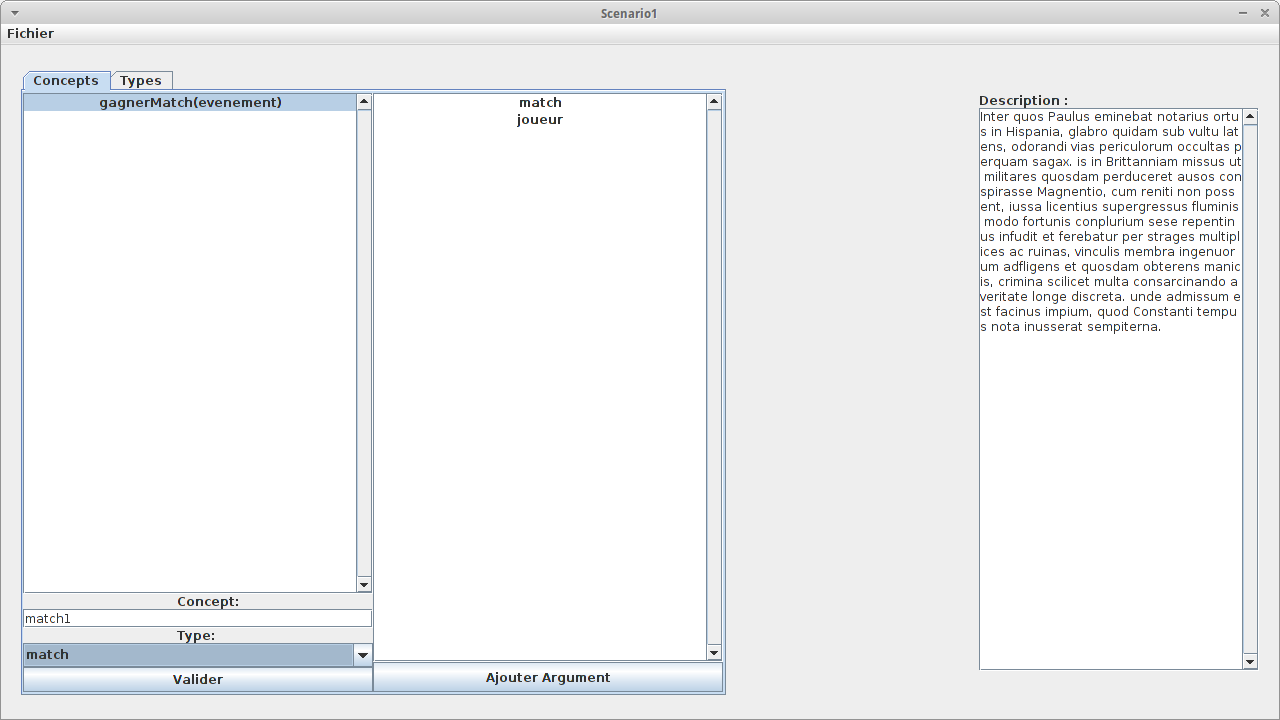
\includegraphics[scale=0.3]{IHM/creation_concepts.png}
\caption{Ecran de création des concepts}
\end{figure}
\begin{figure}
\centering
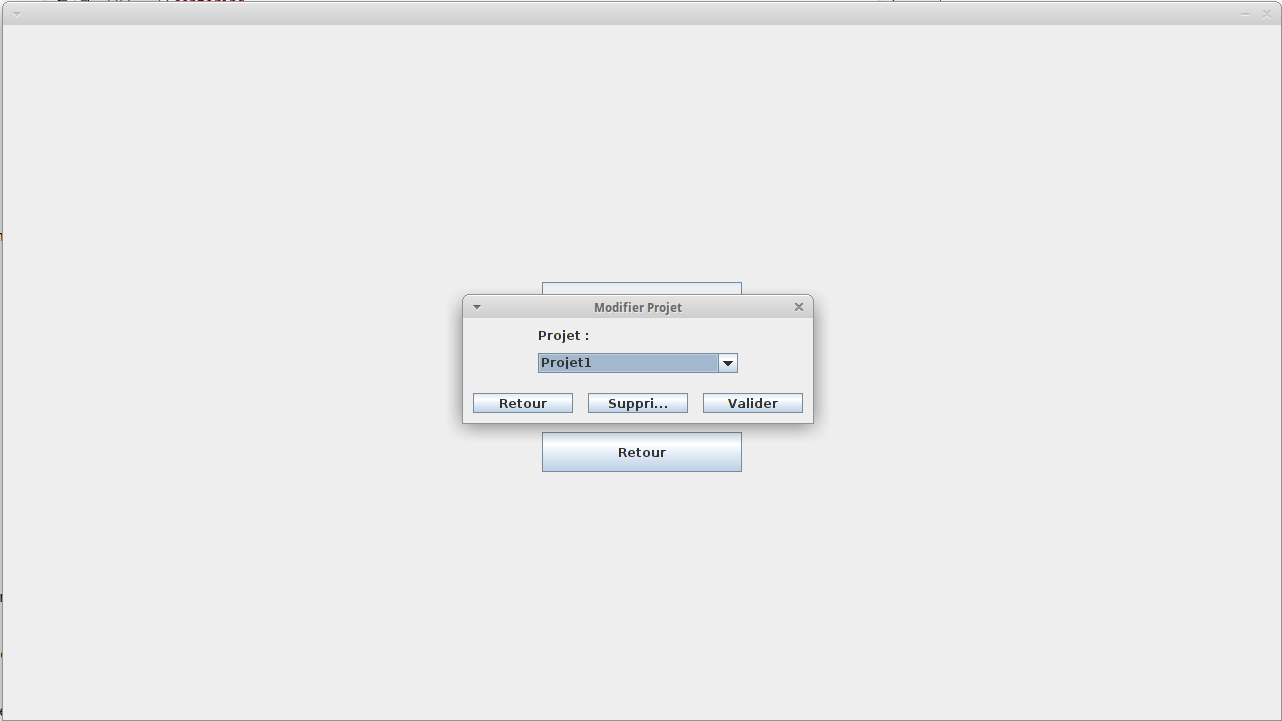
\includegraphics[scale=0.3]{IHM/modifier_projet_admin.png}
\caption{Ecran de choix du projet à modifier}
\end{figure}
\begin{figure}
\centering
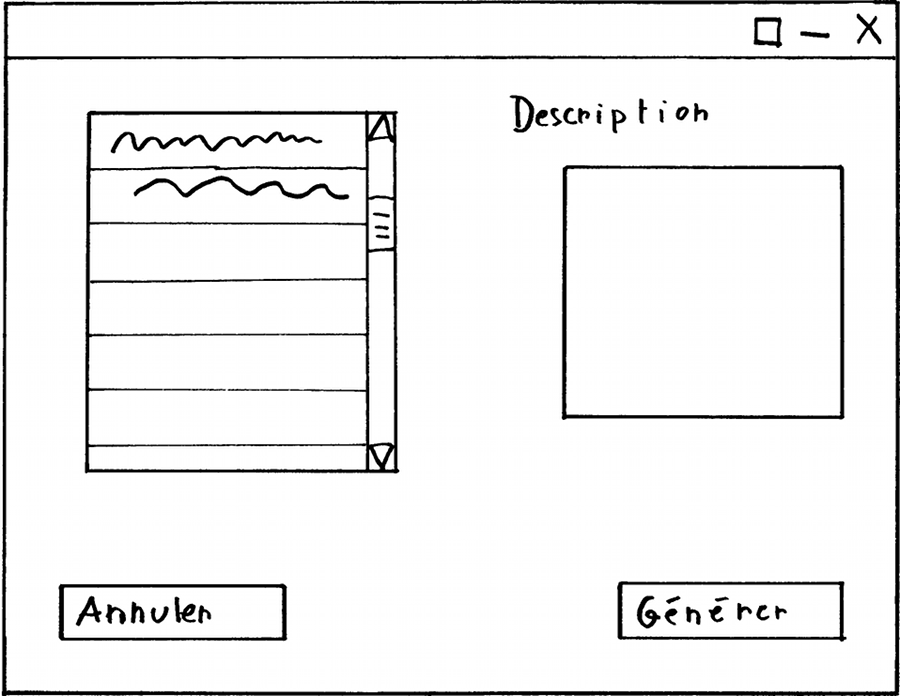
\includegraphics[scale=0.25]{Generation.png}
\caption{Ecran de choix des attributs}
\end{figure}

\chapter{Tests et résultats}
\section{Tests effectués}
Le but de ces tests est d'assurer le bon fonctionnement de notre application. Nous pouvons les regrouper selon l'ensemble de fonctionnalités auquels ils se rattachent. Afin de ne pas mélanger le code source et les essais, nous avons créé un package différent regroupant l'ensemble des classes et méthodes de test. 

\subsection{Package Linguistique}
Ce package regroupe les principaux objets utilisés par l'interface graphique tels que les concepts, graphes, noeuds et système de typage des concepts. Son bon fonctionnement était donc primordial pour ne pas avoir d'erreurs lors de l'utilisation de ces derniers par l'interface graphique. Nous avons donc élaboré des tests unitaires, au moyen de JUnit, sur chacune des classes et méthodes. 
\begin{itemize}	
\item ConceptTest : Dans les classes Concept(Abstract/Complex/Simple) nous rappelons qu'il y a majoritairement des accesseurs mais également des méthodes utilisées pour la génération de l'entrée Syntox. Notons que les accesseurs ne sont normalement pas des éléments soulevant des problèmes. Toutefois nous nous sommes assurés que les éléments retournés sont bien ceux attendus, surtout dans le cas de la liste et du nombre d'éléments qu'elle contient.
Concernant la méthode generateSyntox() nous avons choisi de la tester lors de l'utilisation d'un objet ``GraphConcepts''.
\begin{figure}
\begin{center}
	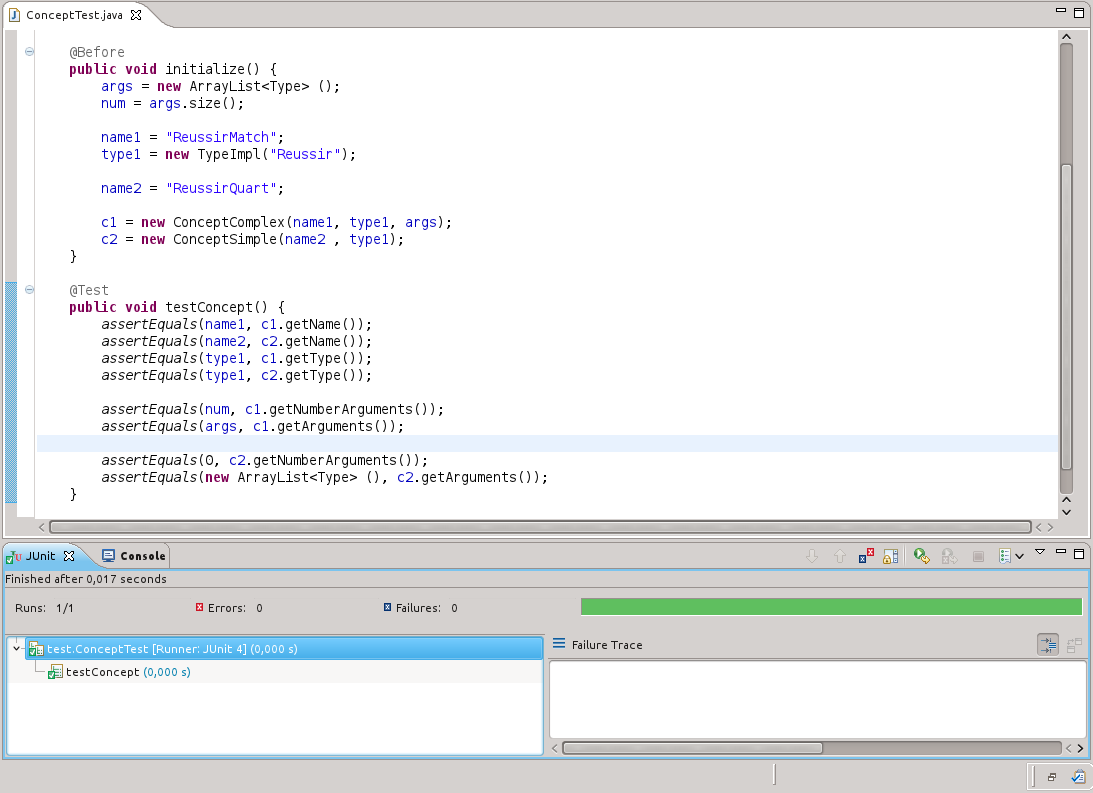
\includegraphics[scale=0.40]{resultatTest1.png}
\end{center}
\end{figure}
\item TypeTest : Nous avons ici testé de manière similaire à "ConceptTest" les accesseurs présents. 
\begin{figure}[h!]
\begin{center}
	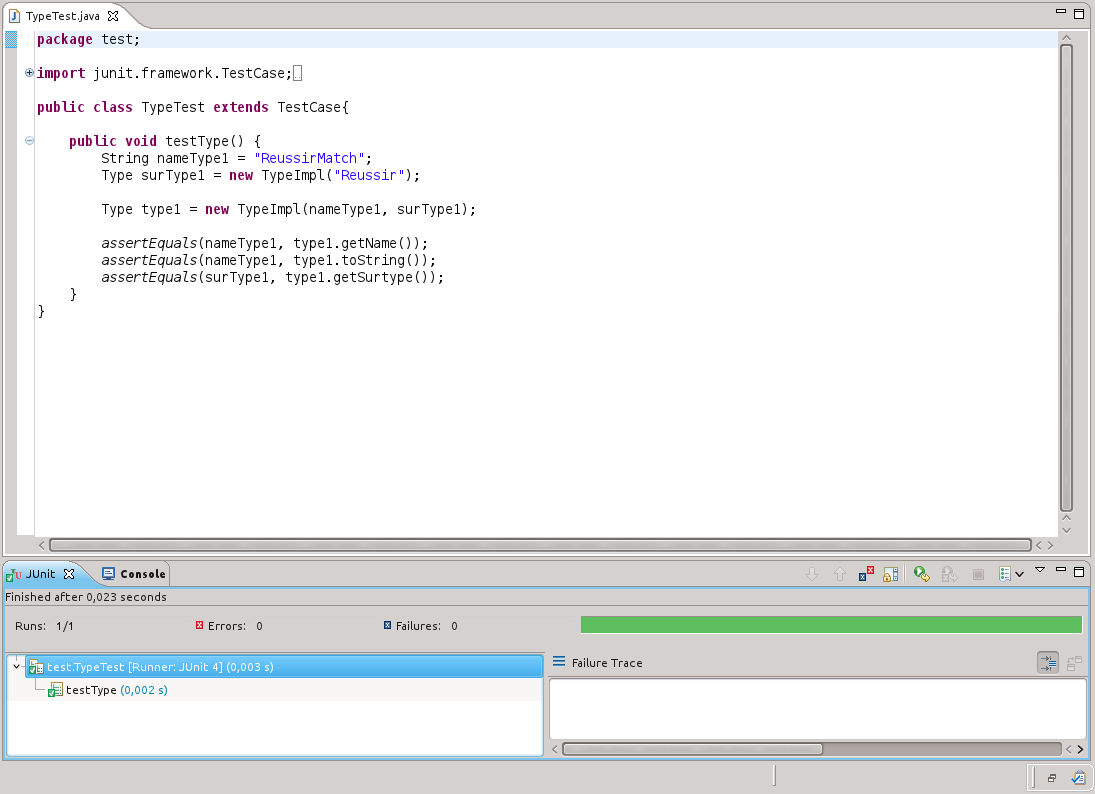
\includegraphics[scale=0.40]{resultatTest6.png}
\end{center}
\end{figure}
\item TypeTreeTest et TypeTreeNodeTest : Nous avons fait le choix de tester l'intégralité des méthodes présentes dans ces classes, à savoir :
	\begin{itemize}
	\item L'ajout d'un nouveau concept à la liste du noeud en question. 
	\item L'ajout d'un fils à la liste concernée.
	\item L'ajout d'un type dans l'objet TypeTree (Plus précisément dans la Map de l'objet) en respectant les liaisons avec un type prédécesseur (surType). Et de façon similaire, l'ajout d'un concept à ce même objet.
	\item La méthode permettant de retourner l'ensemble des sous-types que contient un type. 
	\end{itemize}
\begin{figure}[h!]
\begin{center}
	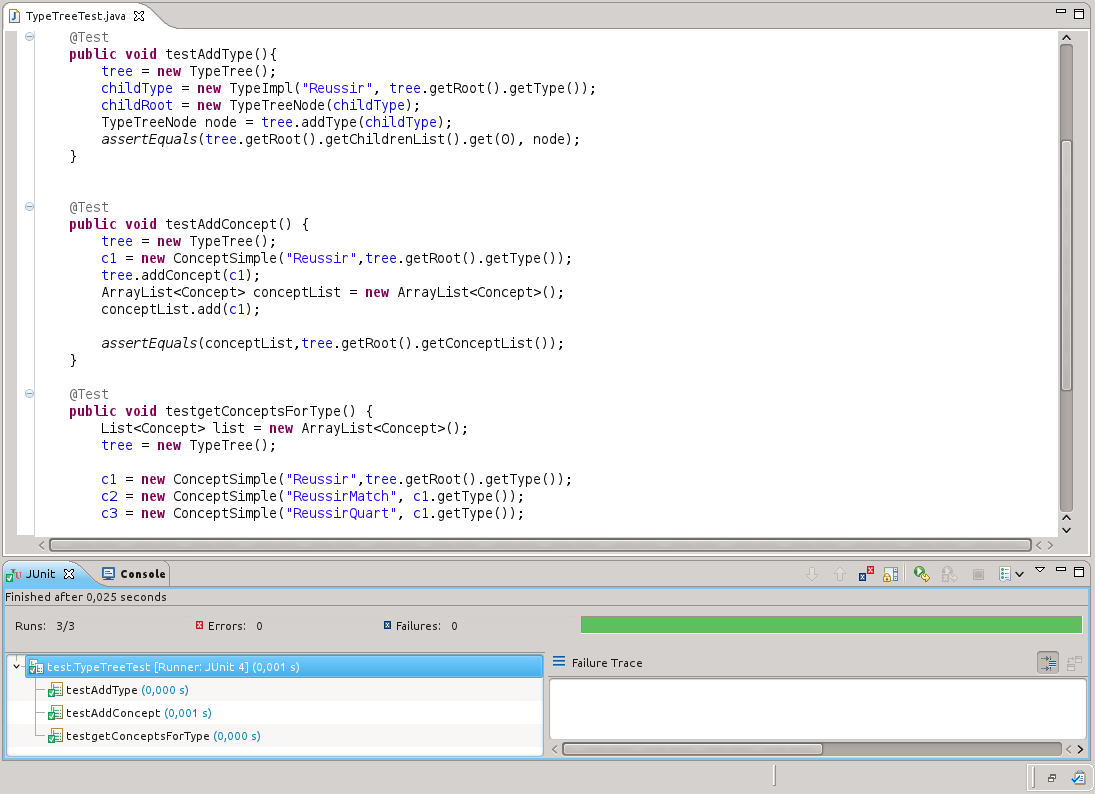
\includegraphics[scale=0.40]{resultatTest8.png}
\end{center}
\end{figure}
\begin{figure}[h!]
\begin{center}
	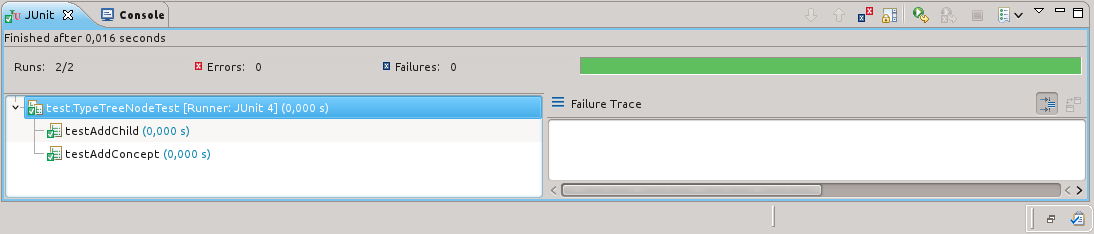
\includegraphics[scale=0.40]{resultatTest7.png}
\end{center}
\end{figure}
\item TypeManagerTest : Nous rappelons que cette classe permet de gérer la création des types ainsi que leur insertion dans l'arbre. 
Nous avons testé la méthode permettant l'ajout d'un type dans l'arbre (makeType() avec un et deux arguments) ainsi que la méthode retournant si deux types sont compatibles (isCompatible()).
\begin{figure}[h!]
\begin{center}
	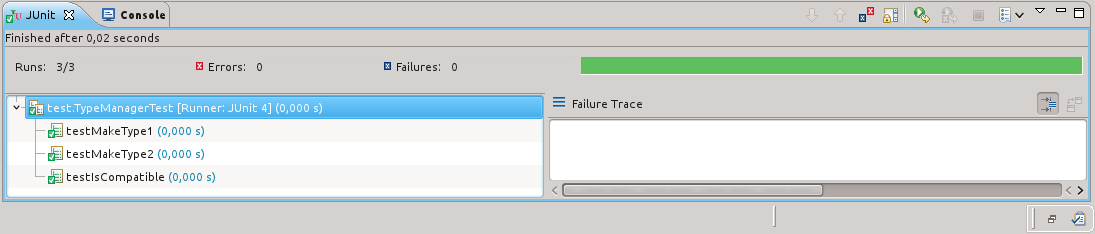
\includegraphics[scale=0.40]{resultatTest5.png}
\end{center}
\end{figure}
\item LinguisticFactoryTest : Nous avons choisi de tester les méthodes qui apportent les fonctionnalités suivantes: 
	\begin{itemize}
	\item L'ajout d'un type au TypeManager au moyen de la méthode ``makeType''.
	\item L'ajout de concept, simple ou complex à l'arbre qu'utilise le TypeManager.
	\end{itemize}
\begin{figure}[h!]
\begin{center}
	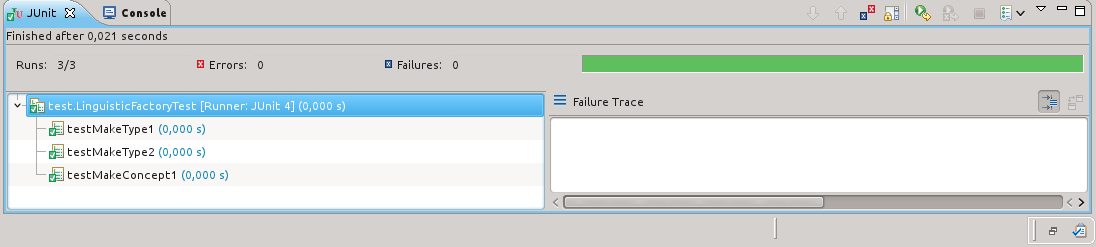
\includegraphics[scale=0.40]{resultatTest4.png}
\end{center}
\end{figure}
\item GraphConceptsTest et GraphNodeDefault: Les classes GraphConcepts et GraphNodeDefault, comme nous le rappelons, permettent la représentation sous forme de graphe des concepts utilisés et sélectionnés par l'utilisateur au moyen de l'interface graphique. 
Nous avons testé pour ces classes :
	\begin{itemize}
	\item Certains accesseurs qui nous semblaient importants dans le sens où ces classes utilisent de nombreux objets d'autres classes, il est donc nécessaire de pouvoir garantir l'accès à ces objets et à leur référence. 
	\item La méthode permettant la création de la requête qui sera envoyée à Syntox (generateSyntox()). Cette méthode est appelée depuis GraphConcepts et fait appel à son homologue présente dans GraphNodeDefault.
	\end{itemize}
\end{itemize}
\begin{figure}[h!]
\begin{center}
	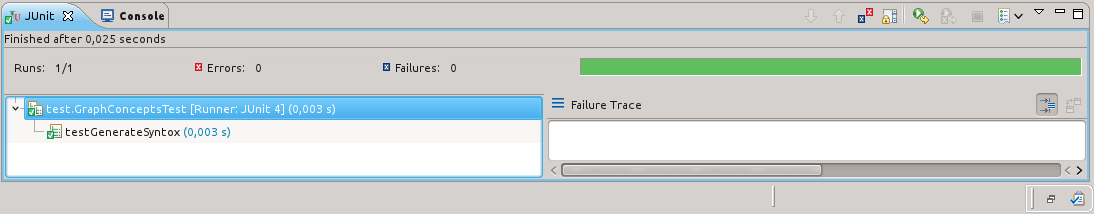
\includegraphics[scale=0.40]{resultatTest2.png}
\end{center}
\end{figure}
\begin{figure}[h!]
\begin{center}
	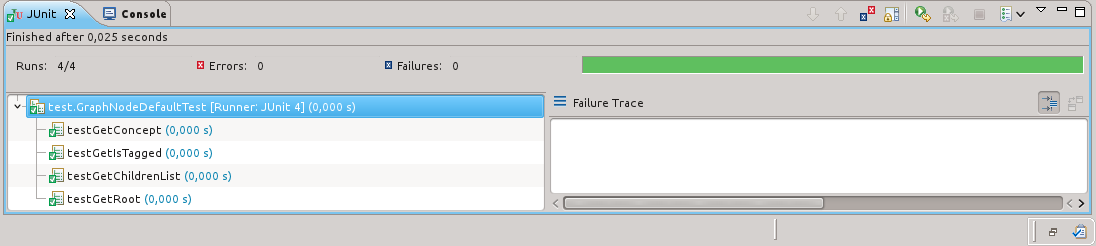
\includegraphics[scale=0.40]{resultatTest3.png}
\end{center}
\end{figure}
\subsection{Core}
	Dans ce package se trouvent toutes les classes permettant le lancement de notre application et les outils nécessaires tel que les éléments permettant la gestion de la sauvegarde des projets, un utilitaire regroupant les informations nécessaires pour la base de données et un système de cryptage/décryptage de mot de passe pour sécuriser l'accès à la base de données. 
Nous avons choisi de tester particulièrement les classes présentes dans les fichiers PasswordManager.java, Project.java et InfoDB.java. Plus précisément nous avons validé les fonctionnalités suivantes :
	\begin{itemize}
	\item L'encryptage ainsi que le décryptage d'un mot de passe. En effet, comme indiqué dans le cahier des besoins, nous ne souhaitons pas laisser le mot de passe utilisé pour la connexion à la base de données en clair. Il nous a donc fallu crypter une fois la connexion faite mais également décrypter si on doit réutiliser le mot de passe.
	\item La conservation des informations saisies pour la base de données au moyen de l'objet initBase. 
	\item L'ajout et la suppression de scénarios relatifs à un Projet.
	\end{itemize}
\subsection{Database[Connection/Inspection]}
\subsection{Syntox}

\subsection{Mémoire et temps de calcul}
	
\section{Résultats}

\chapter{Conclusion et perspectives}


\bibliographystyle{plain}
\bibliography{biblio}

\end{document}
